\documentclass[]{beamer}

\usetheme{Warsaw}
\usecolortheme{whale}
\usepackage{graphicx}
\usepackage{float}

\title{Client-Side Many-Valued \protect\\ Context Scaling}
\author[]{Sebastian Benner}
\institute[]{FB16\\Universität Kassel}

\begin{document}
	\frame{\titlepage}
	
	\AtBeginSection[]
	{
		\begin{frame}
			\frametitle{Table of Contents}
			\tableofcontents[currentsection]
		\end{frame}
	}
	
	\begin{frame}
		\frametitle{Table of Contents}
		\tableofcontents[]
	\end{frame}

	\section[]{Task}

	\begin{frame}
		\frametitle{Task}
		From the website:
		\newline
		\newline
		\begin{quote}
		"Um Datensätze mit z.B. numerischen oder ordinalen Einträgen mit Methoden der Formalen Begriffsanalyse untersuchen zu können, müssen diese zuerst in eine entsprechende Form gebracht (also skaliert) werden. In diesem Projekt soll ein interaktives Tool erstellt werden, mit dem Datensätze begrifflich skaliert werden können."
		\end{quote}
	\end{frame}

	\section[]{Design}

	\begin{frame}
		\frametitle{Initial Draft}
		\begin{figure}[H]
			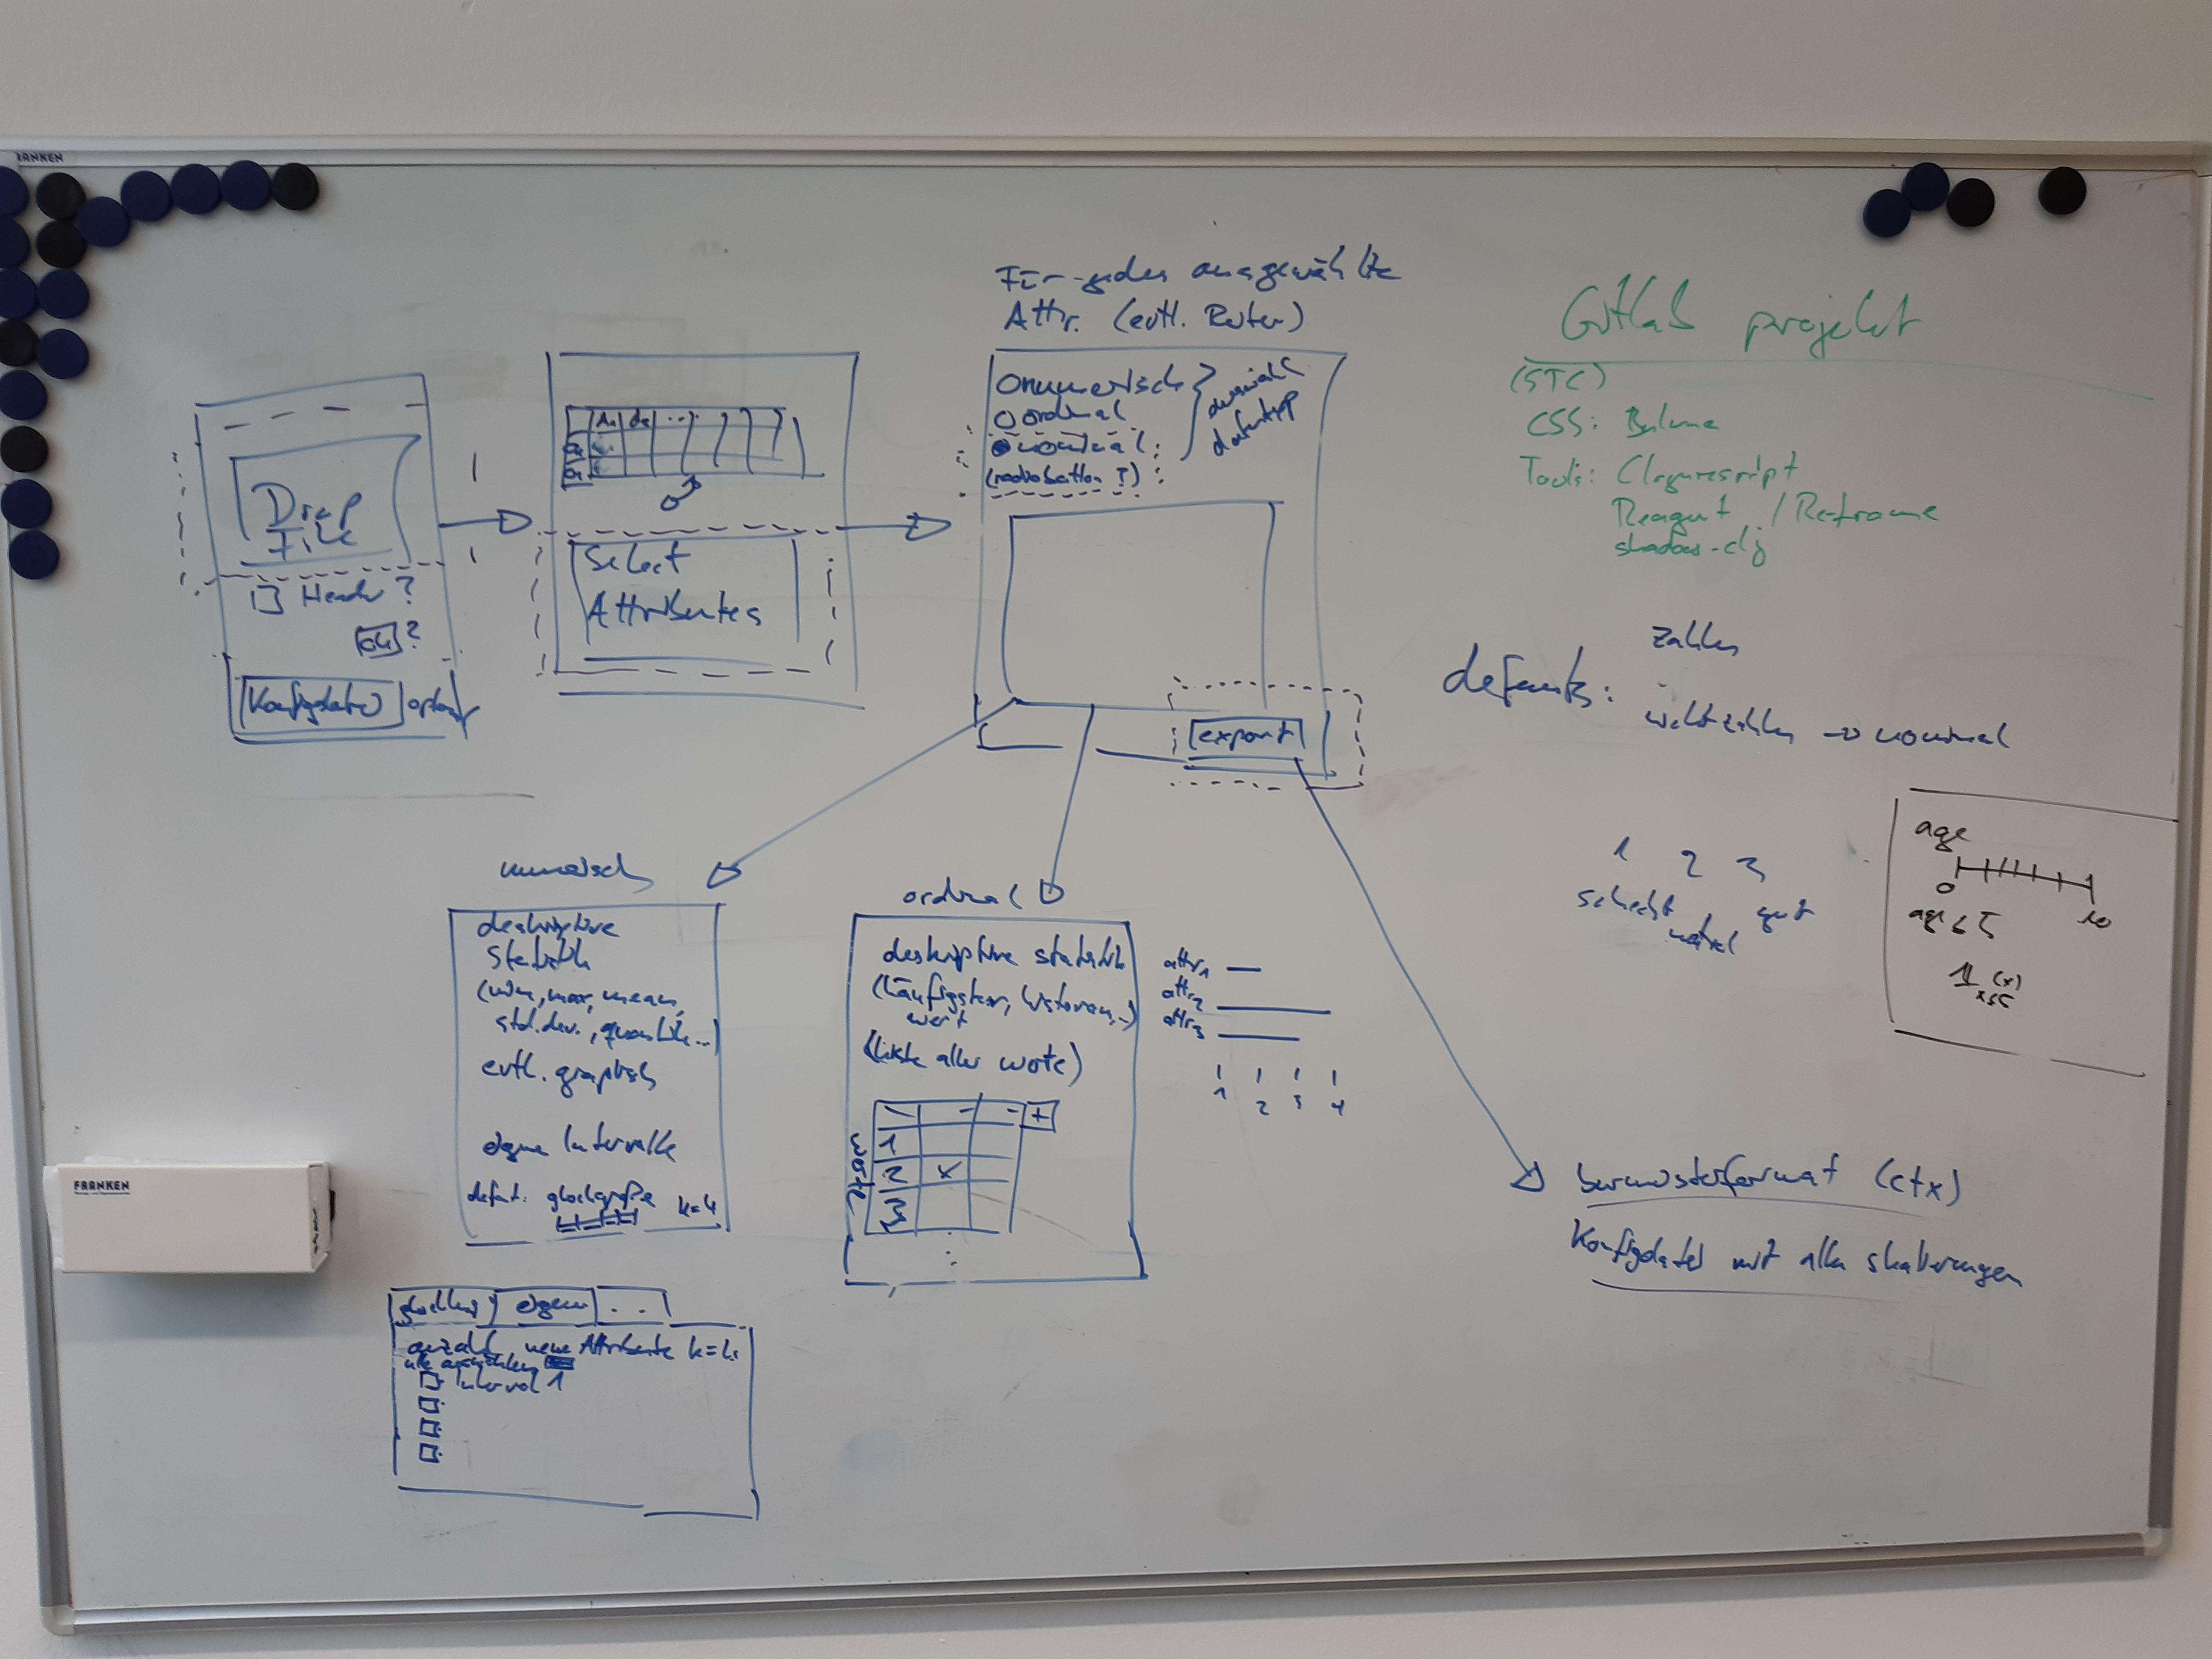
\includegraphics[width=\linewidth]{../mock_up/draft_masterprojekt_whiteboardbild.jpg}
			\label{fig:p1}
		\end{figure}
	\end{frame}

	\begin{frame}
		\frametitle{Initial Draft}
		\begin{figure}[H]
			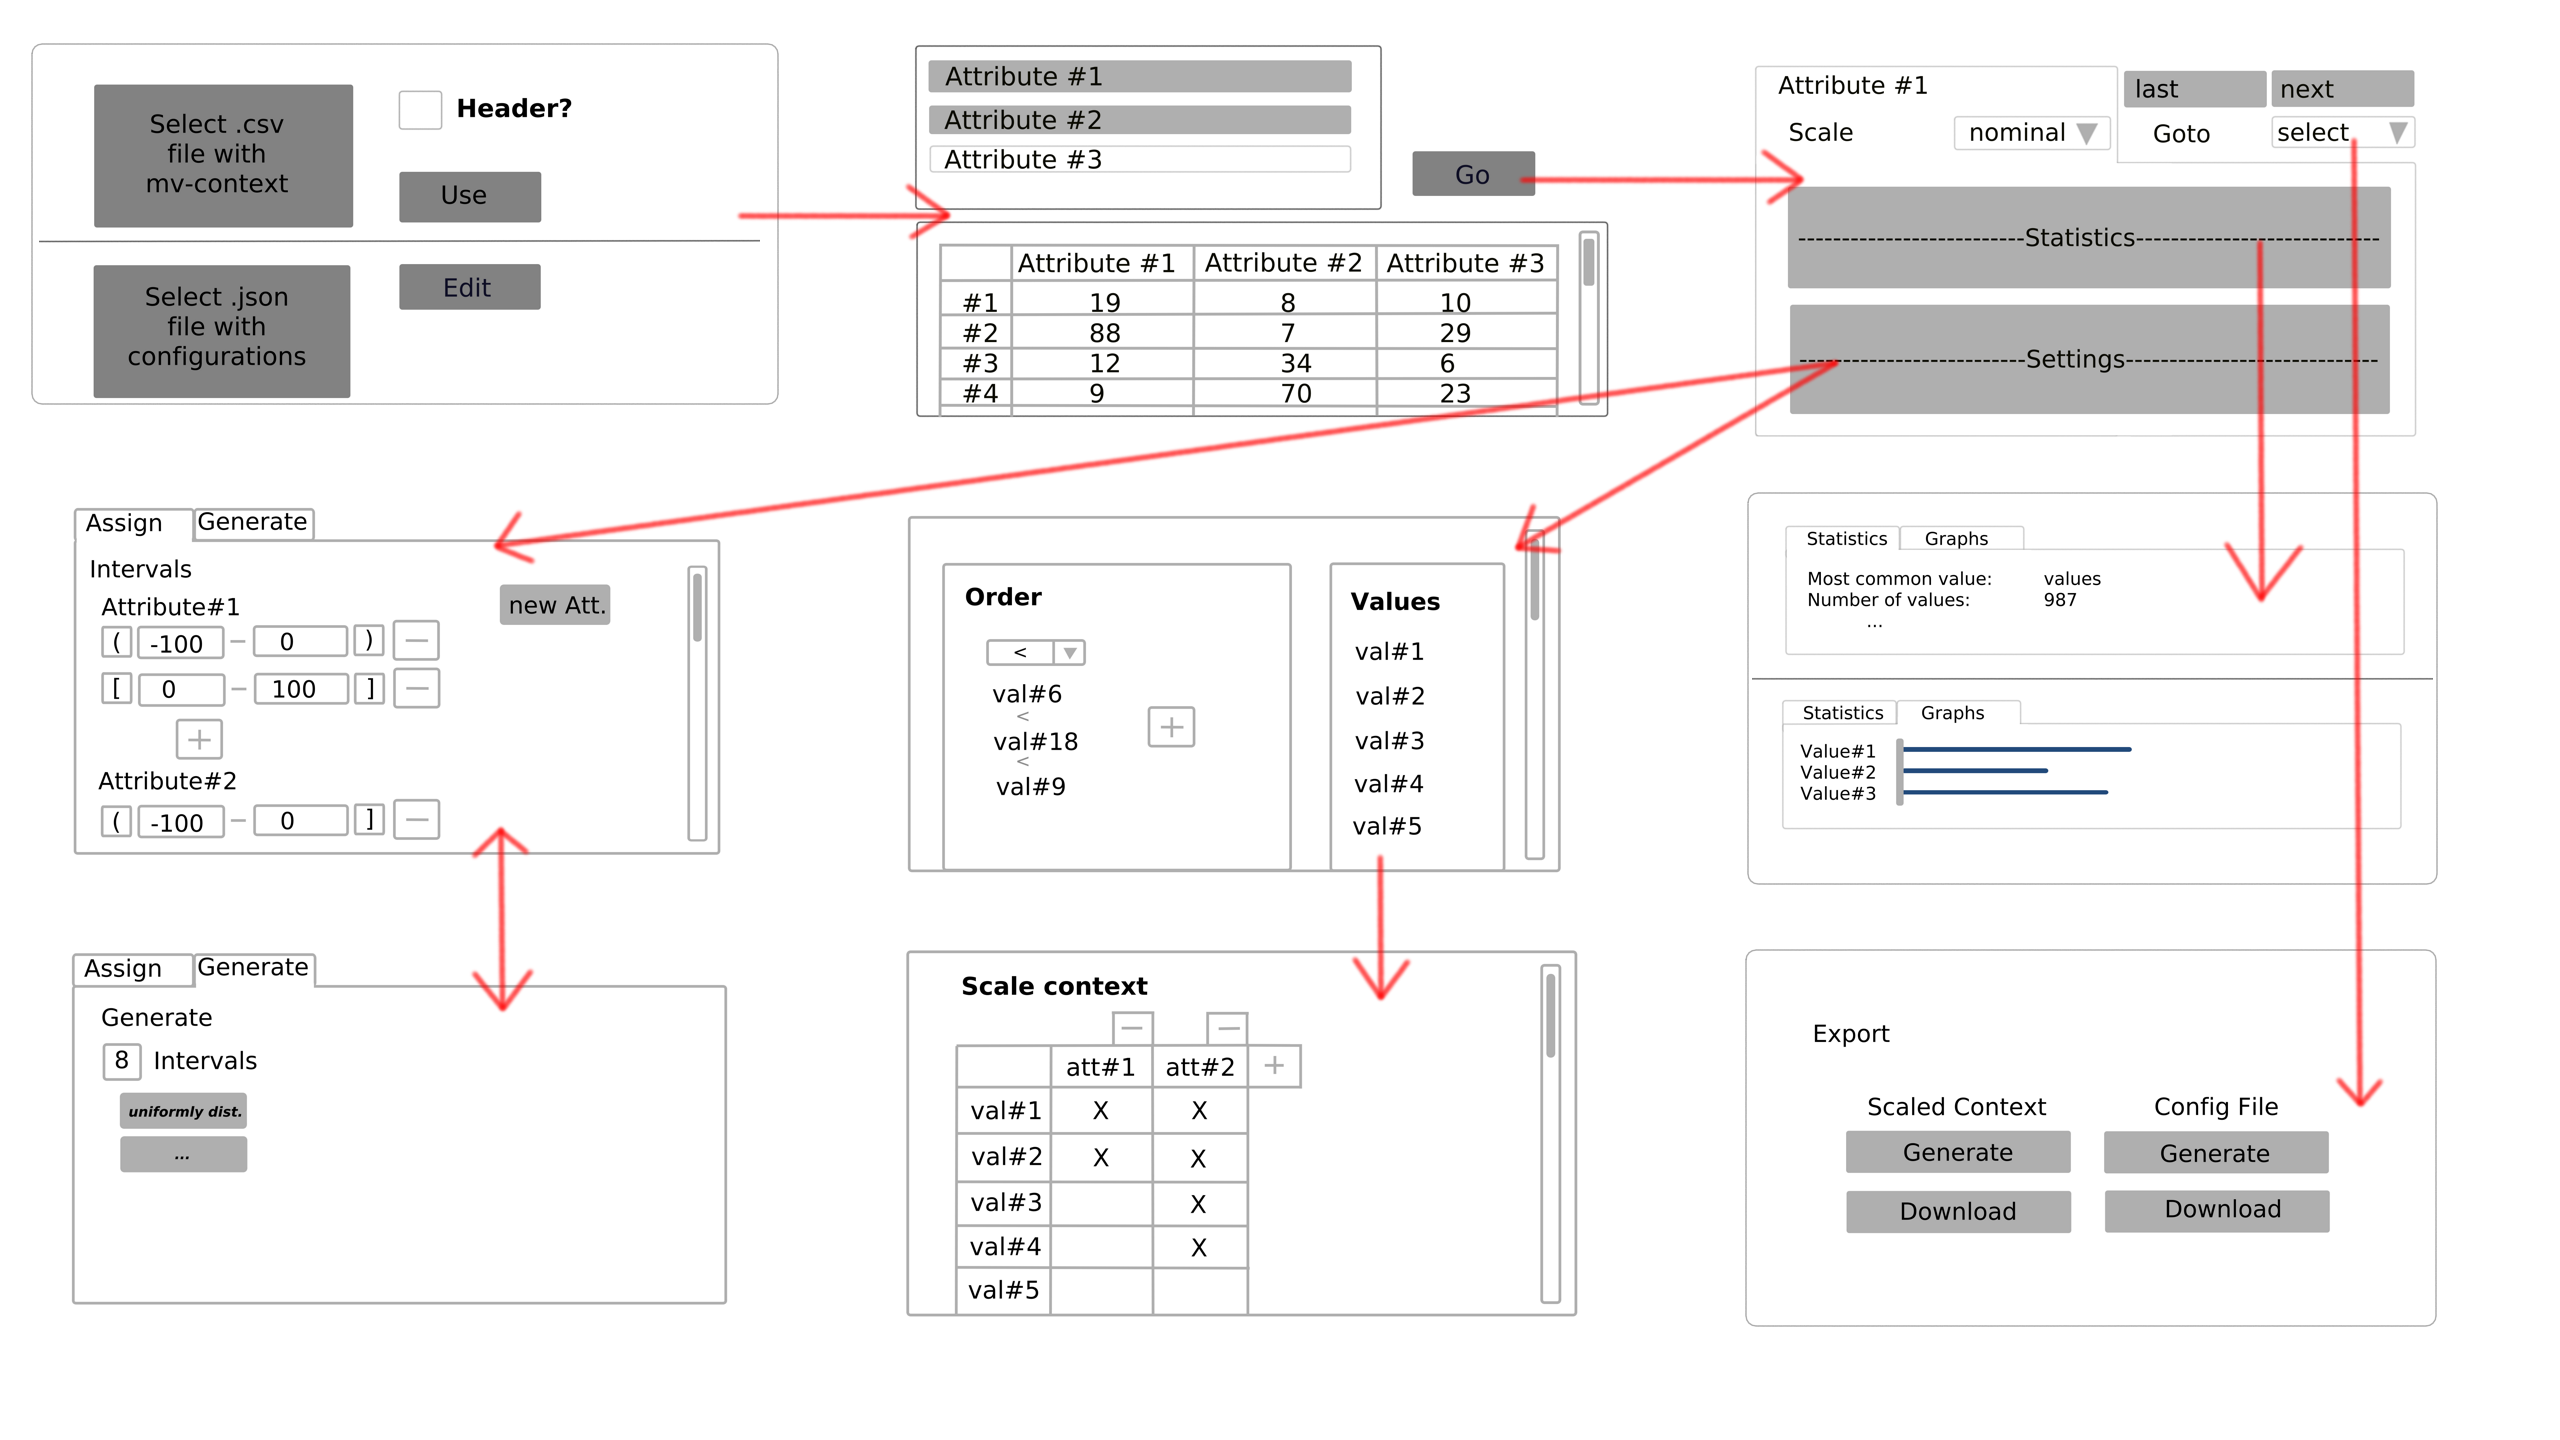
\includegraphics[width=\linewidth]{../mock_up/combi.png}
			\label{fig:p1}
		\end{figure}
	\end{frame}

	\begin{frame}
		\frametitle{Upload}
		\begin{figure}[H]
			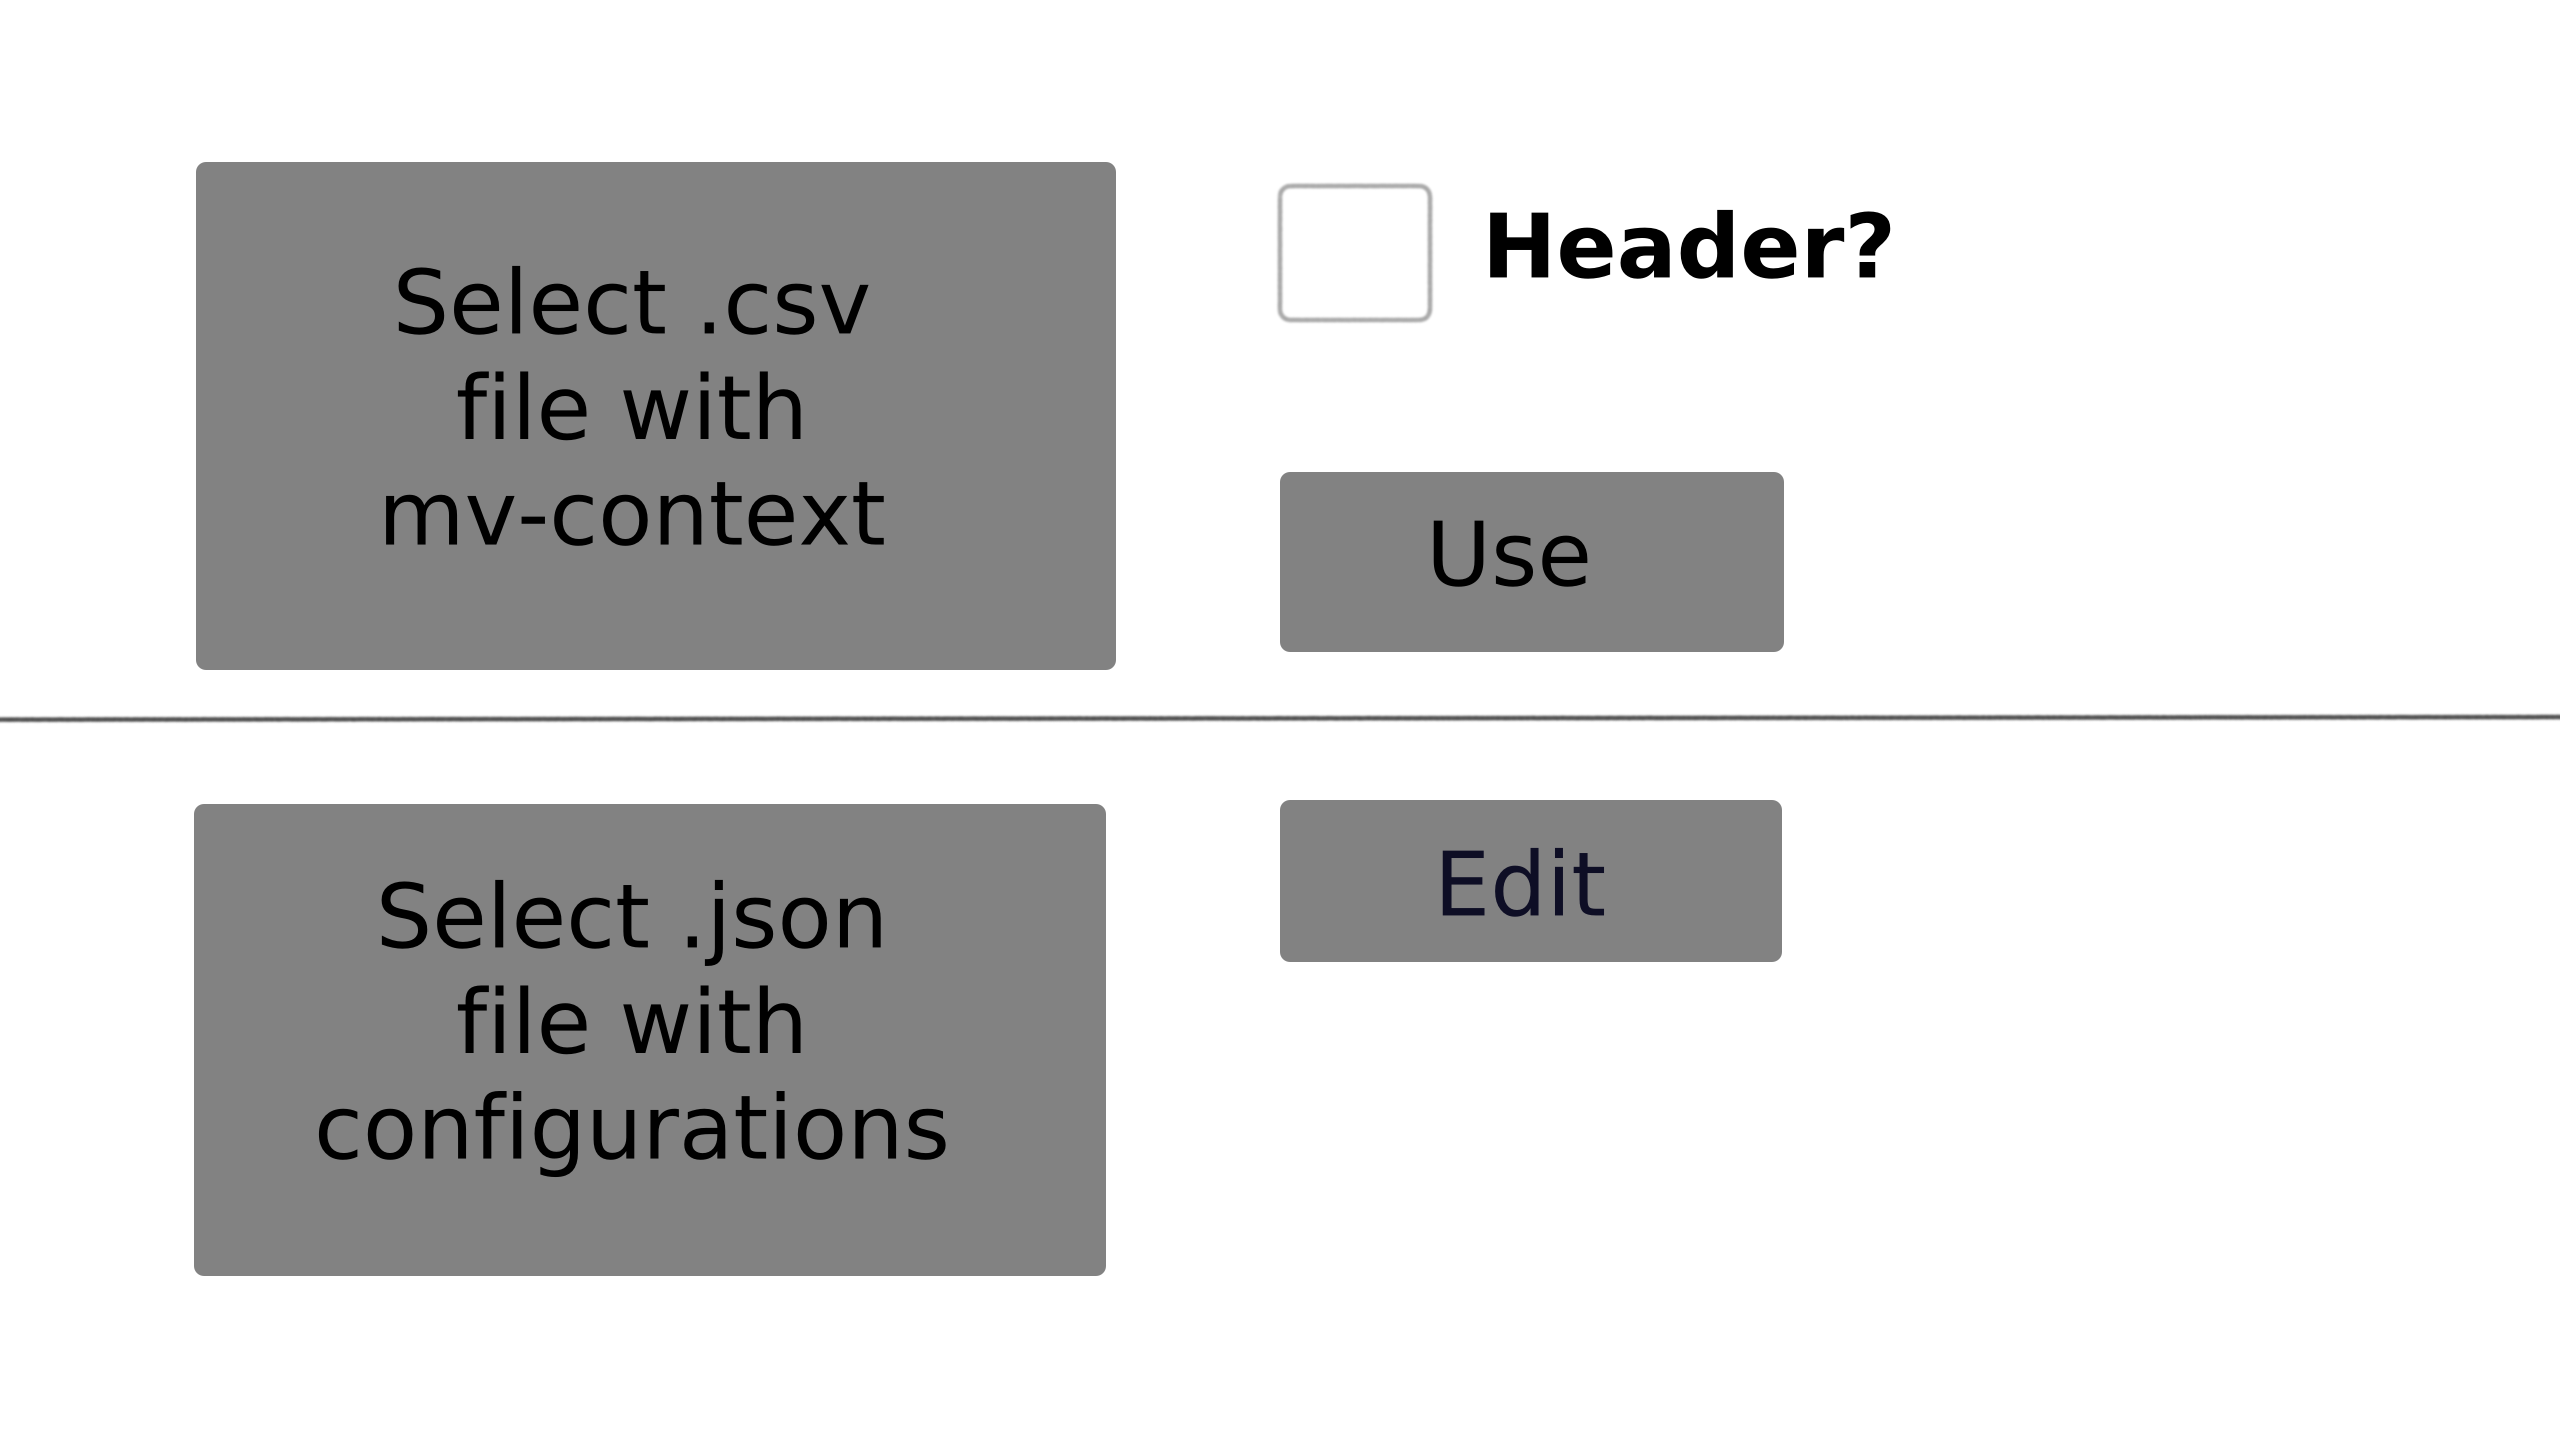
\includegraphics[width=\linewidth]{../mock_up/panel-1.png}
			\caption{Select files to upload}
			\label{fig:p1}
		\end{figure}
	\end{frame}

	\begin{frame}
		\frametitle{Select attributes}
		\begin{figure}[H]
			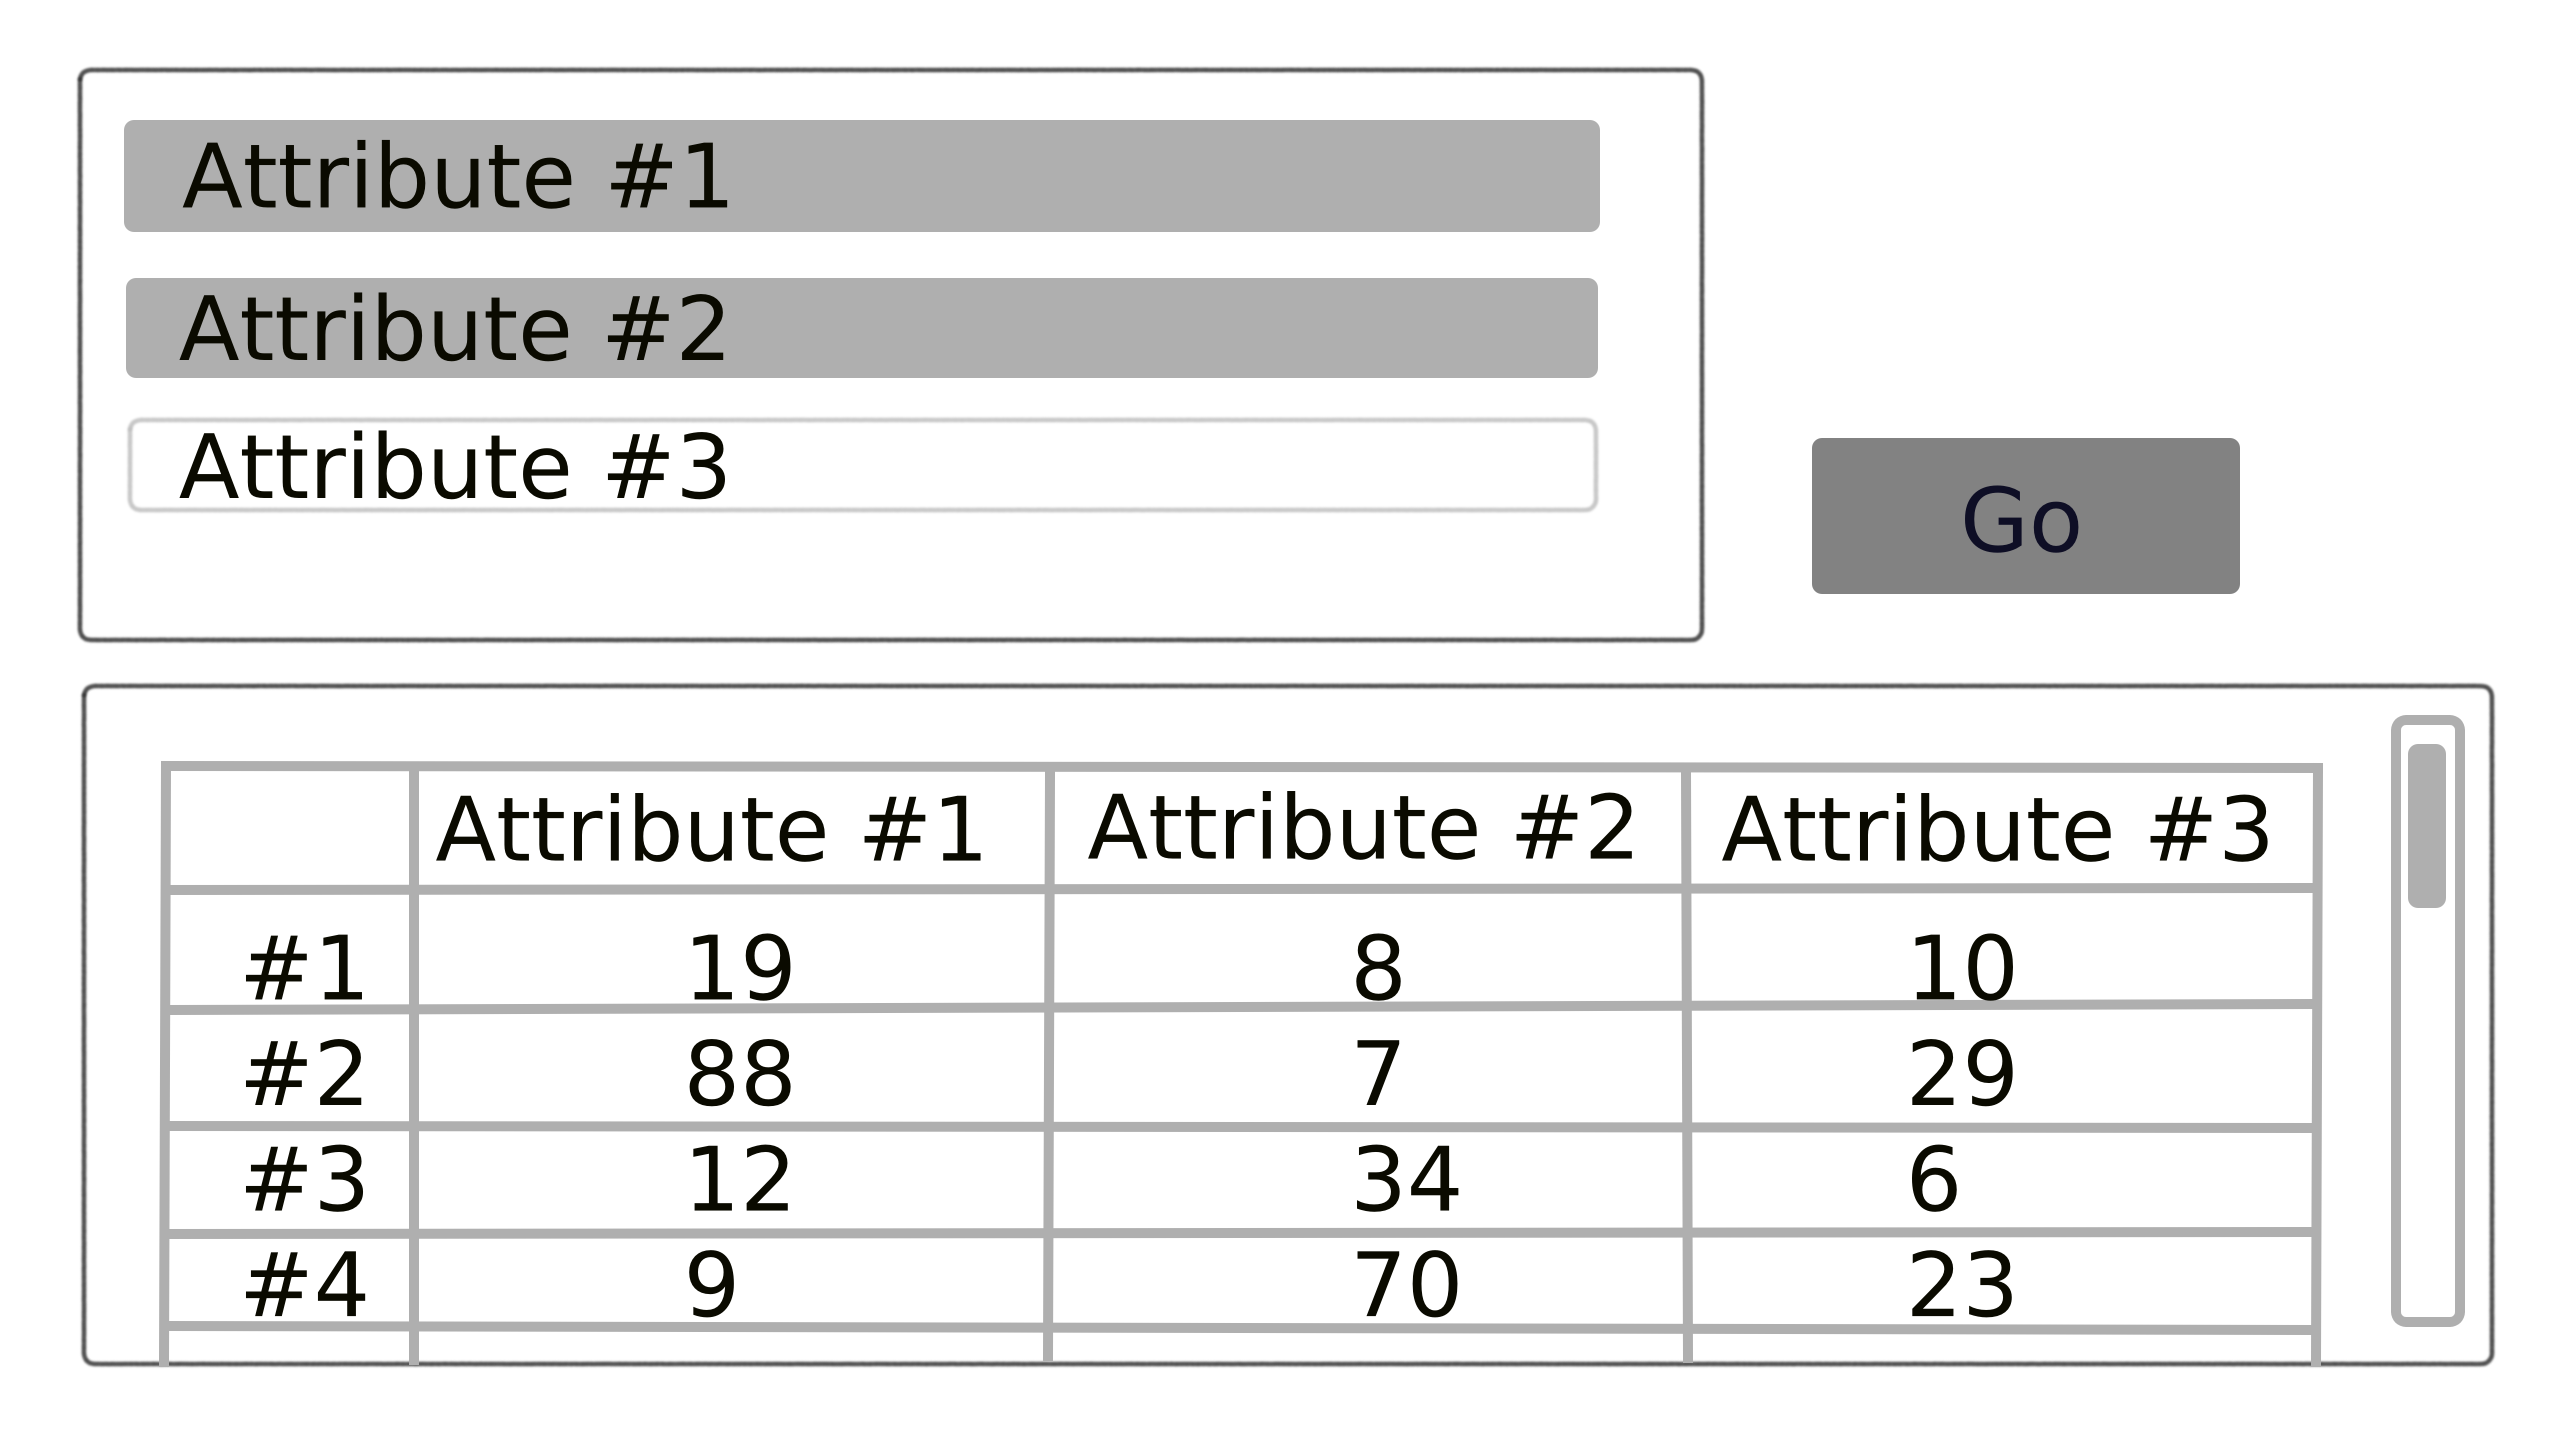
\includegraphics[width=\linewidth]{../mock_up/panel-2.png}
			\caption{Select attributes to scale}
			\label{fig:p1}
		\end{figure}
	\end{frame}

	\begin{frame}
		\frametitle{Actual scaling}
		\begin{figure}[H]
			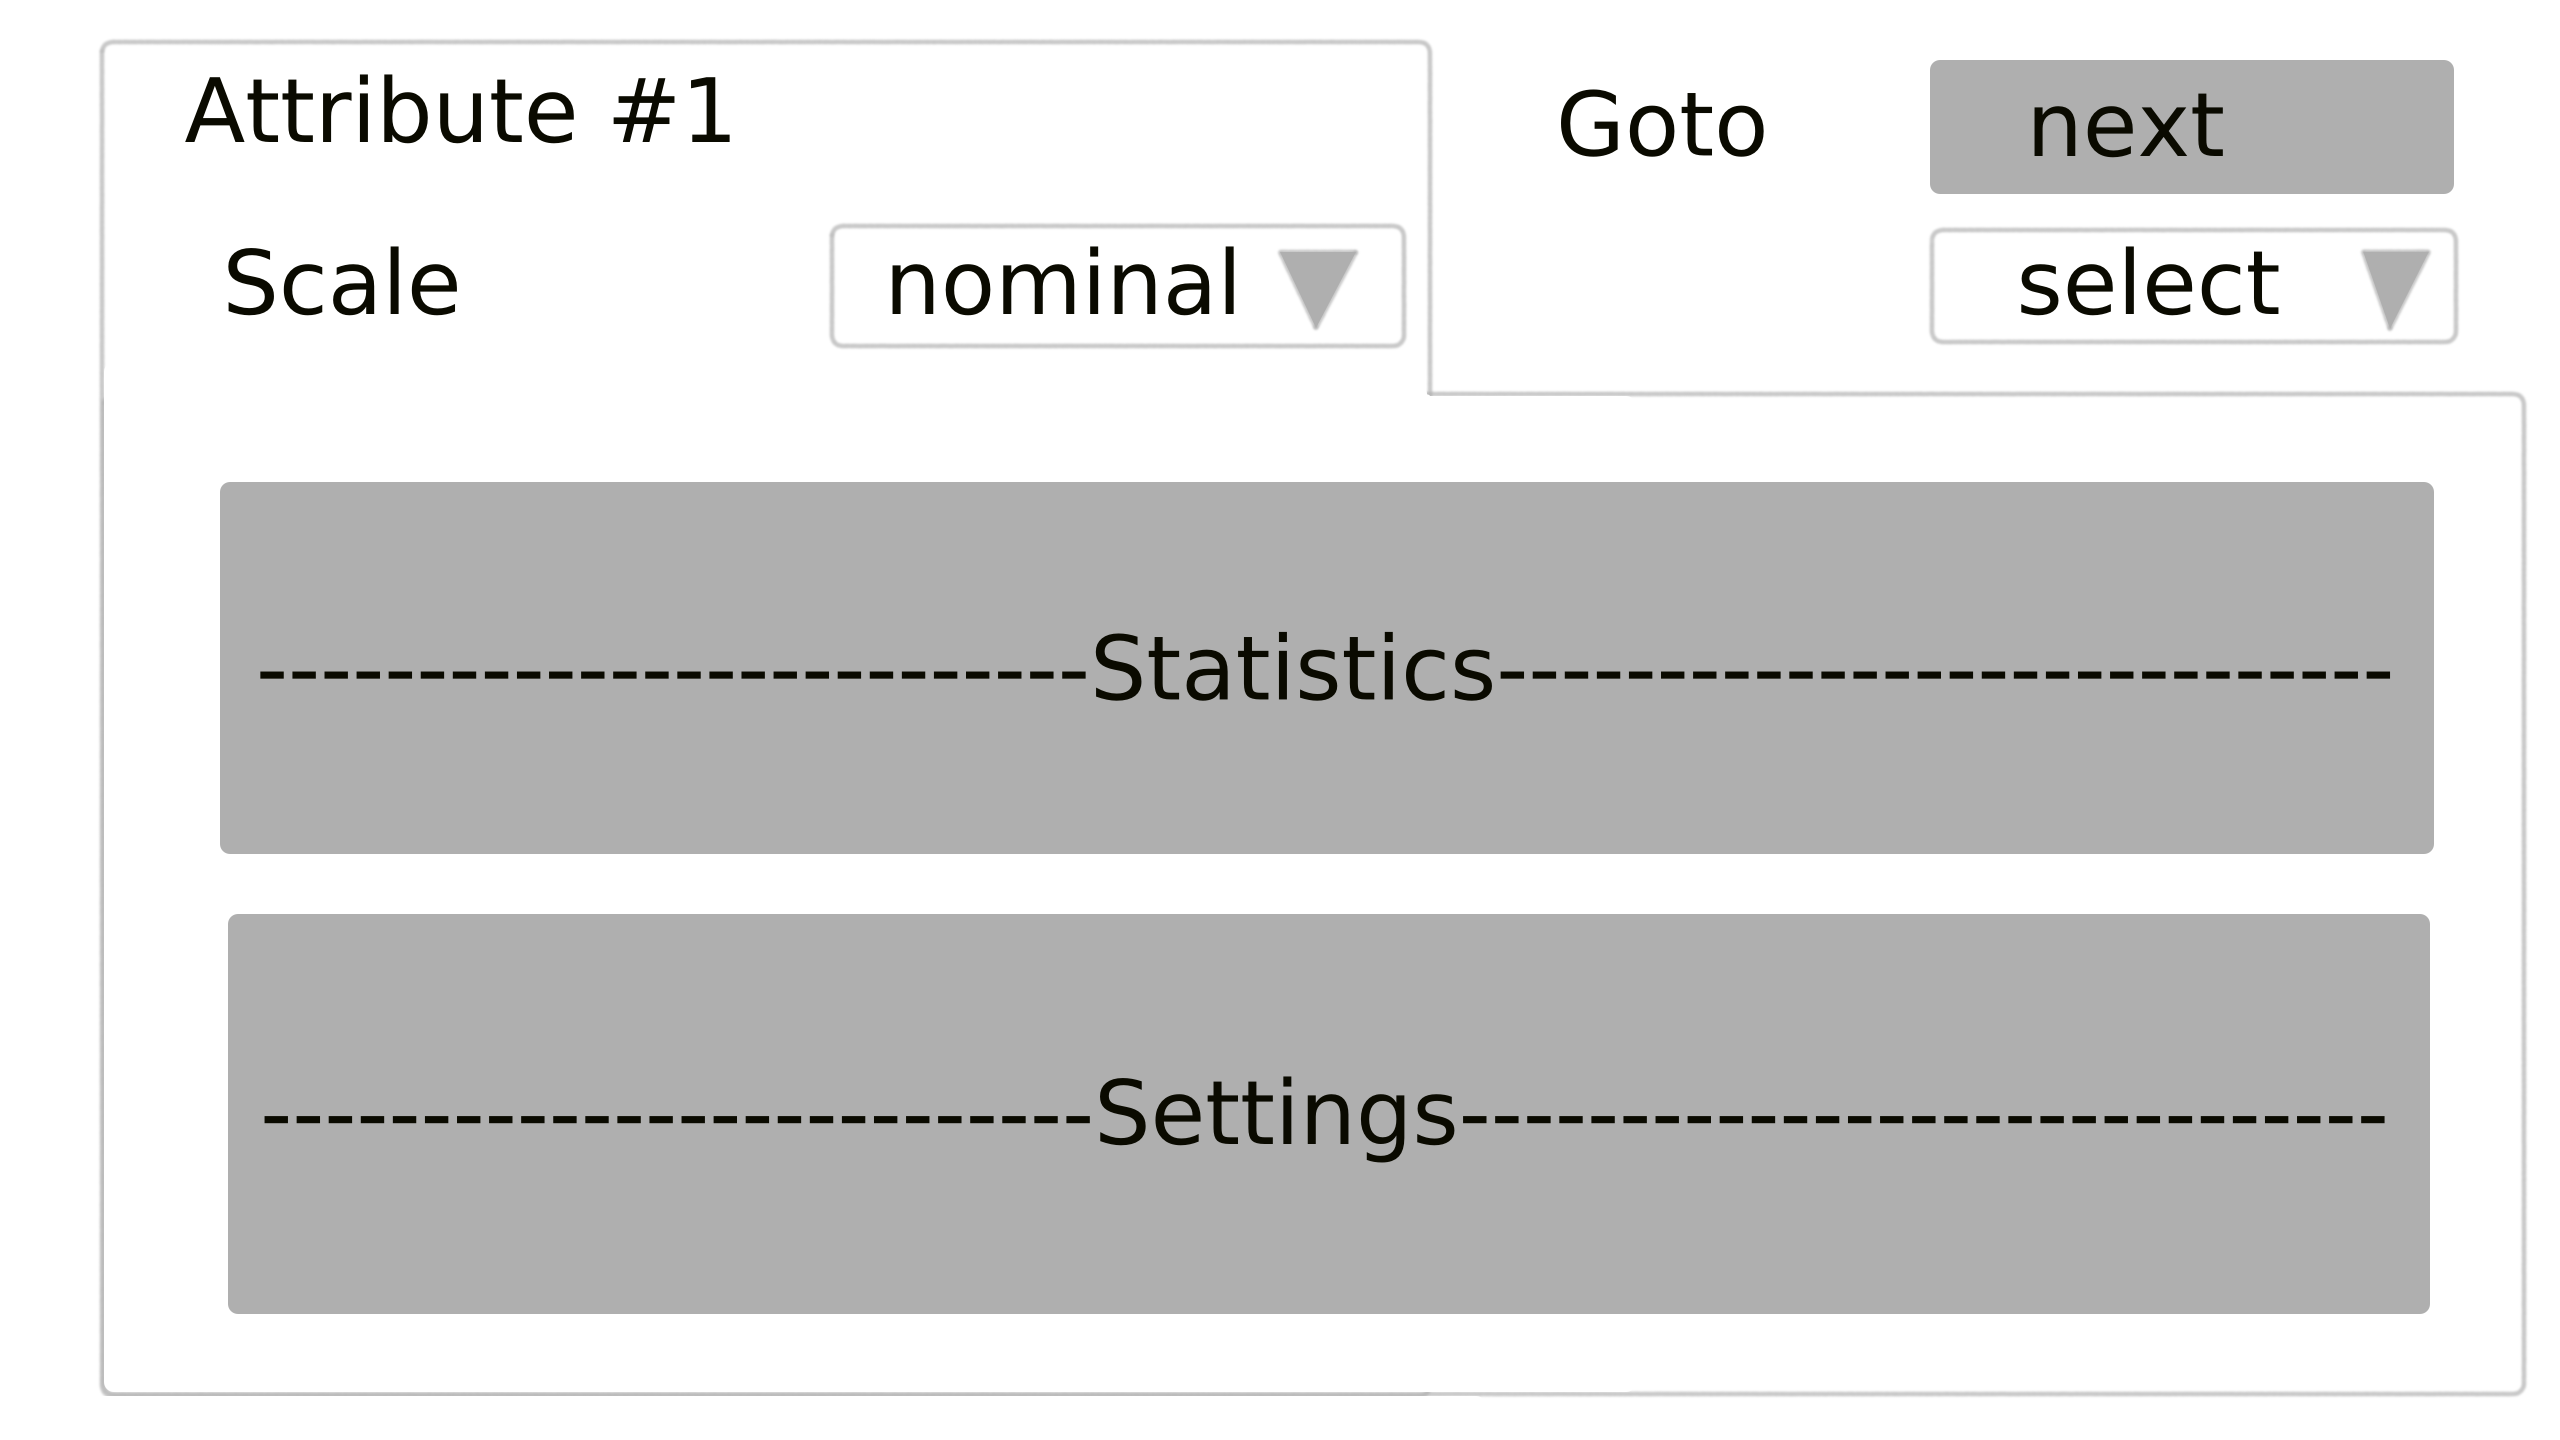
\includegraphics[width=\linewidth]{../mock_up/panel-3.png}
			\caption{For each attribute, select the scaling}
			\label{fig:p1}
		\end{figure}
	\end{frame}

	\begin{frame}
		\frametitle{Statistics}
		\begin{figure}[H]
			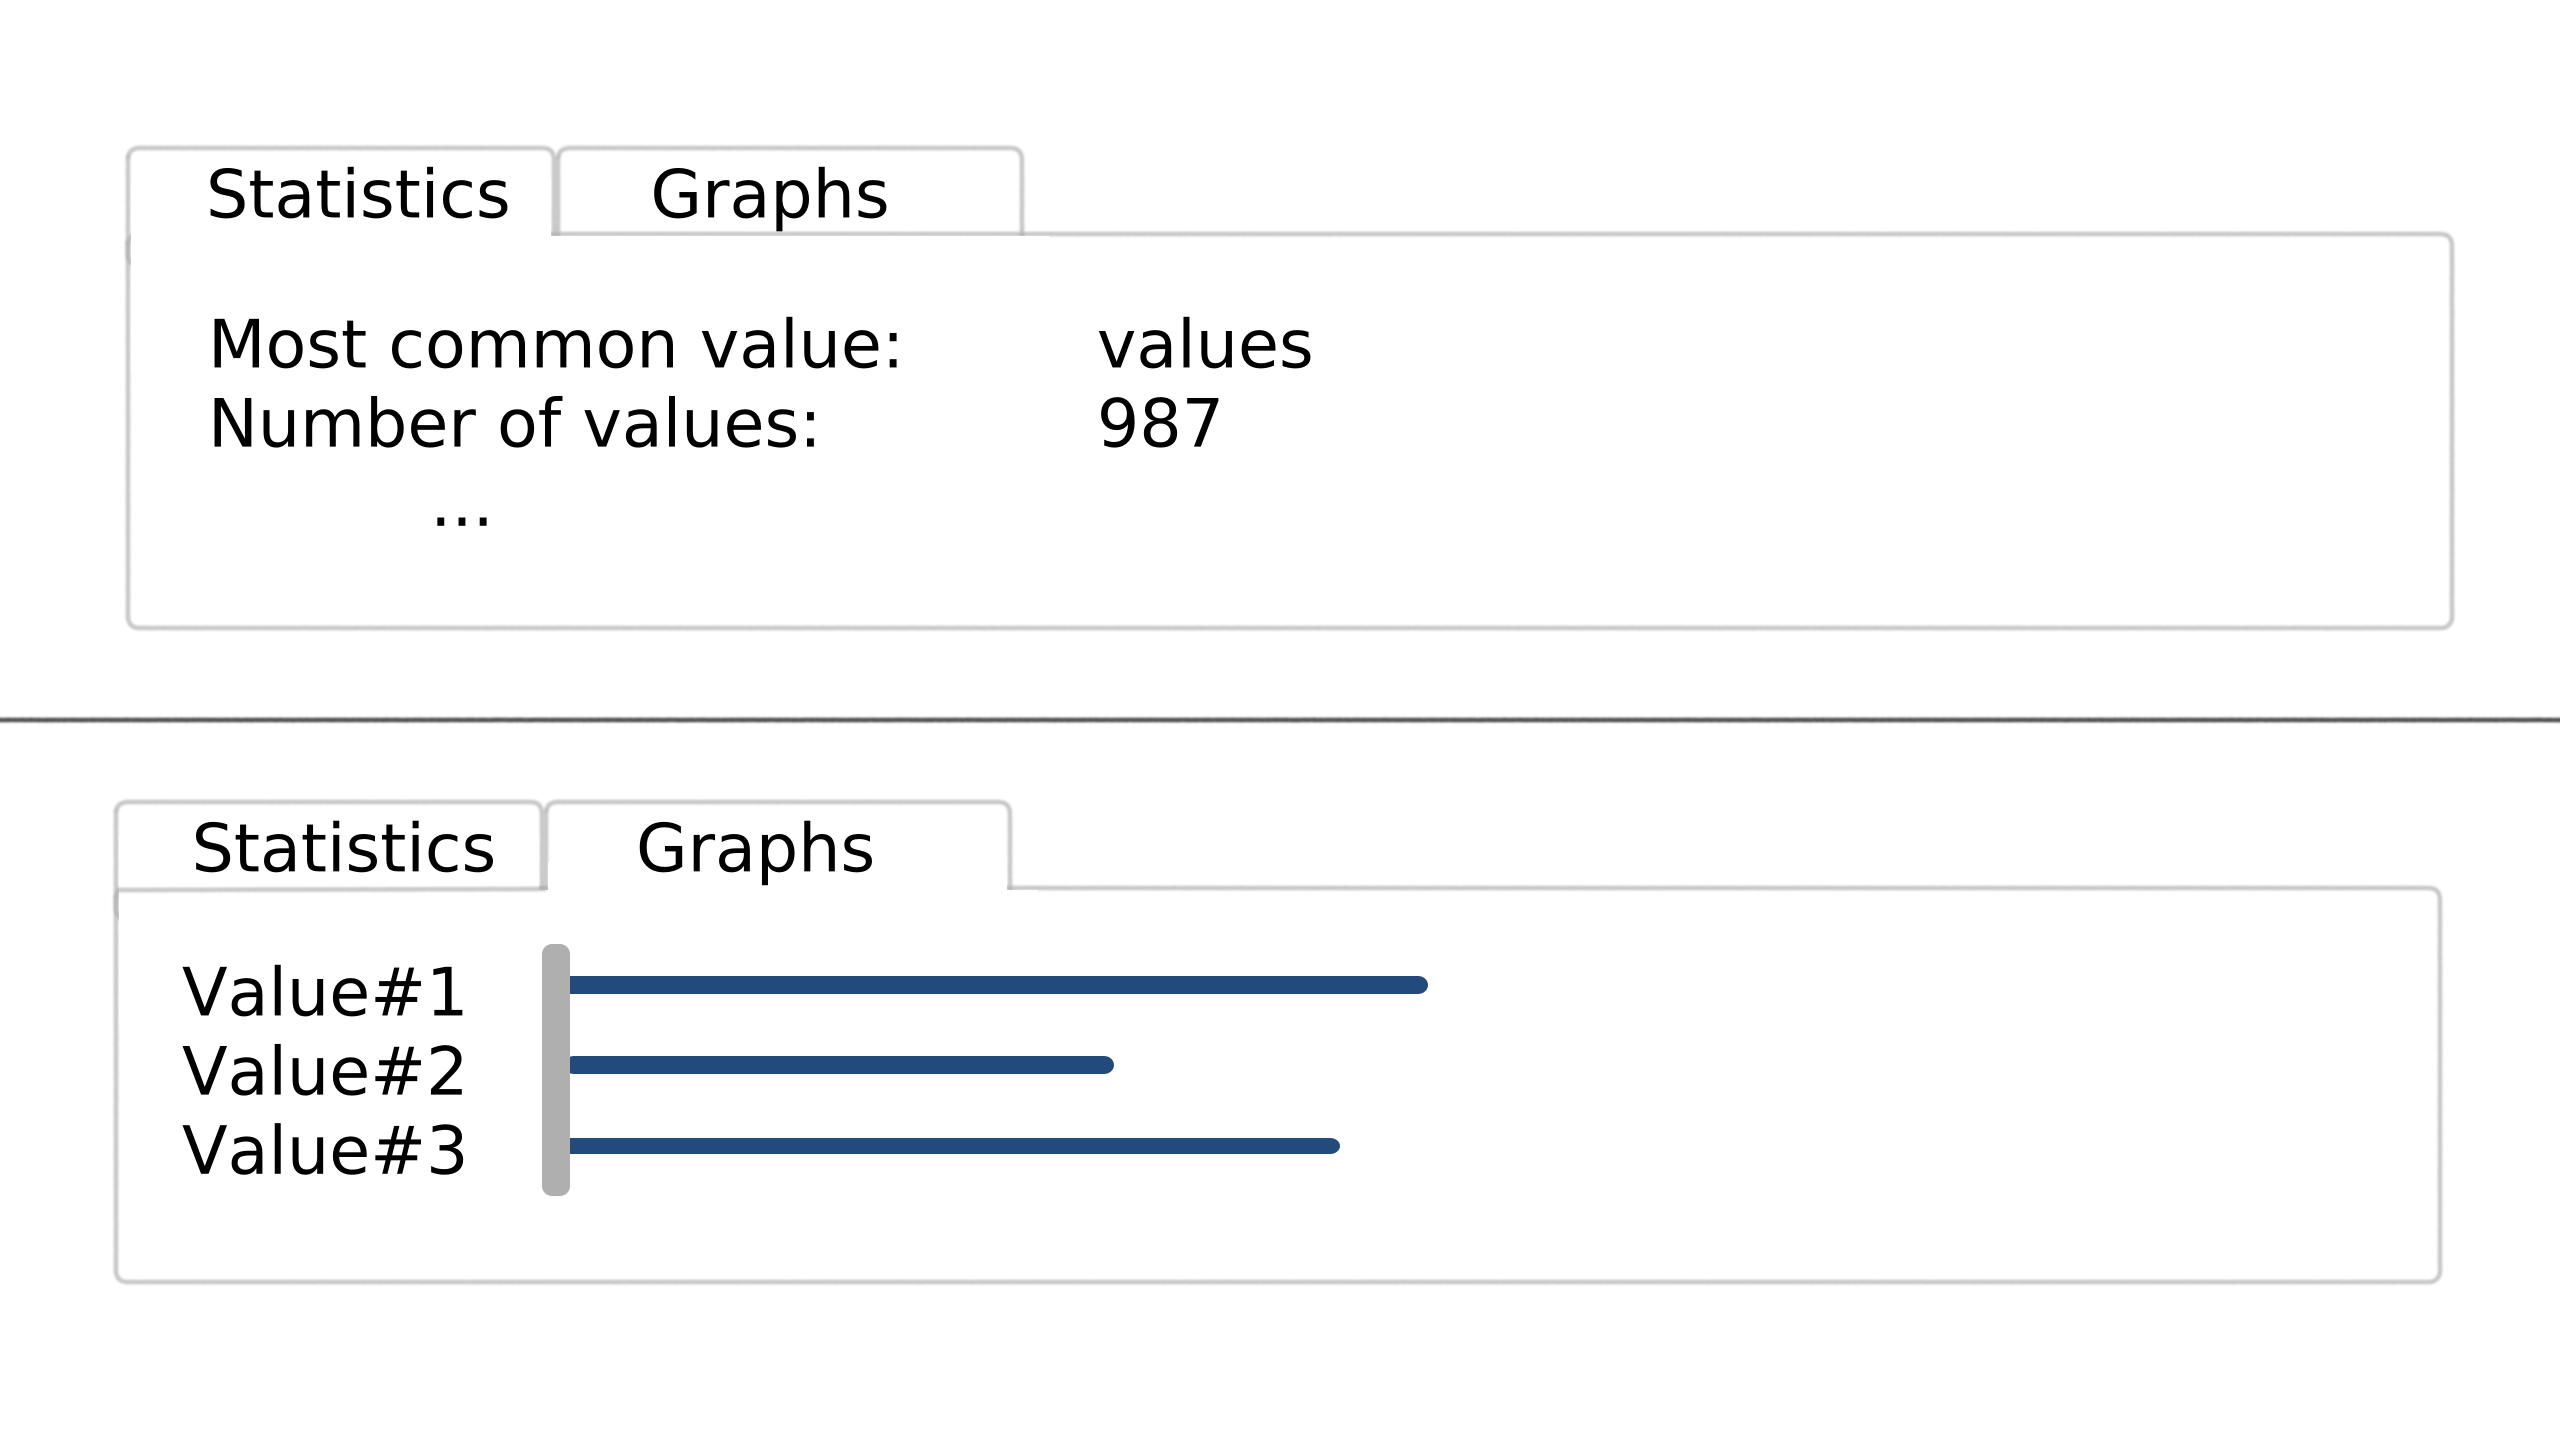
\includegraphics[width=\linewidth]{../mock_up/stat.png}
			\caption{Some statistics based on chosen measure}
			\label{fig:p1}
		\end{figure}
	\end{frame}

	\begin{frame}
		\frametitle{Ordinal scaling}
		\begin{figure}[H]
			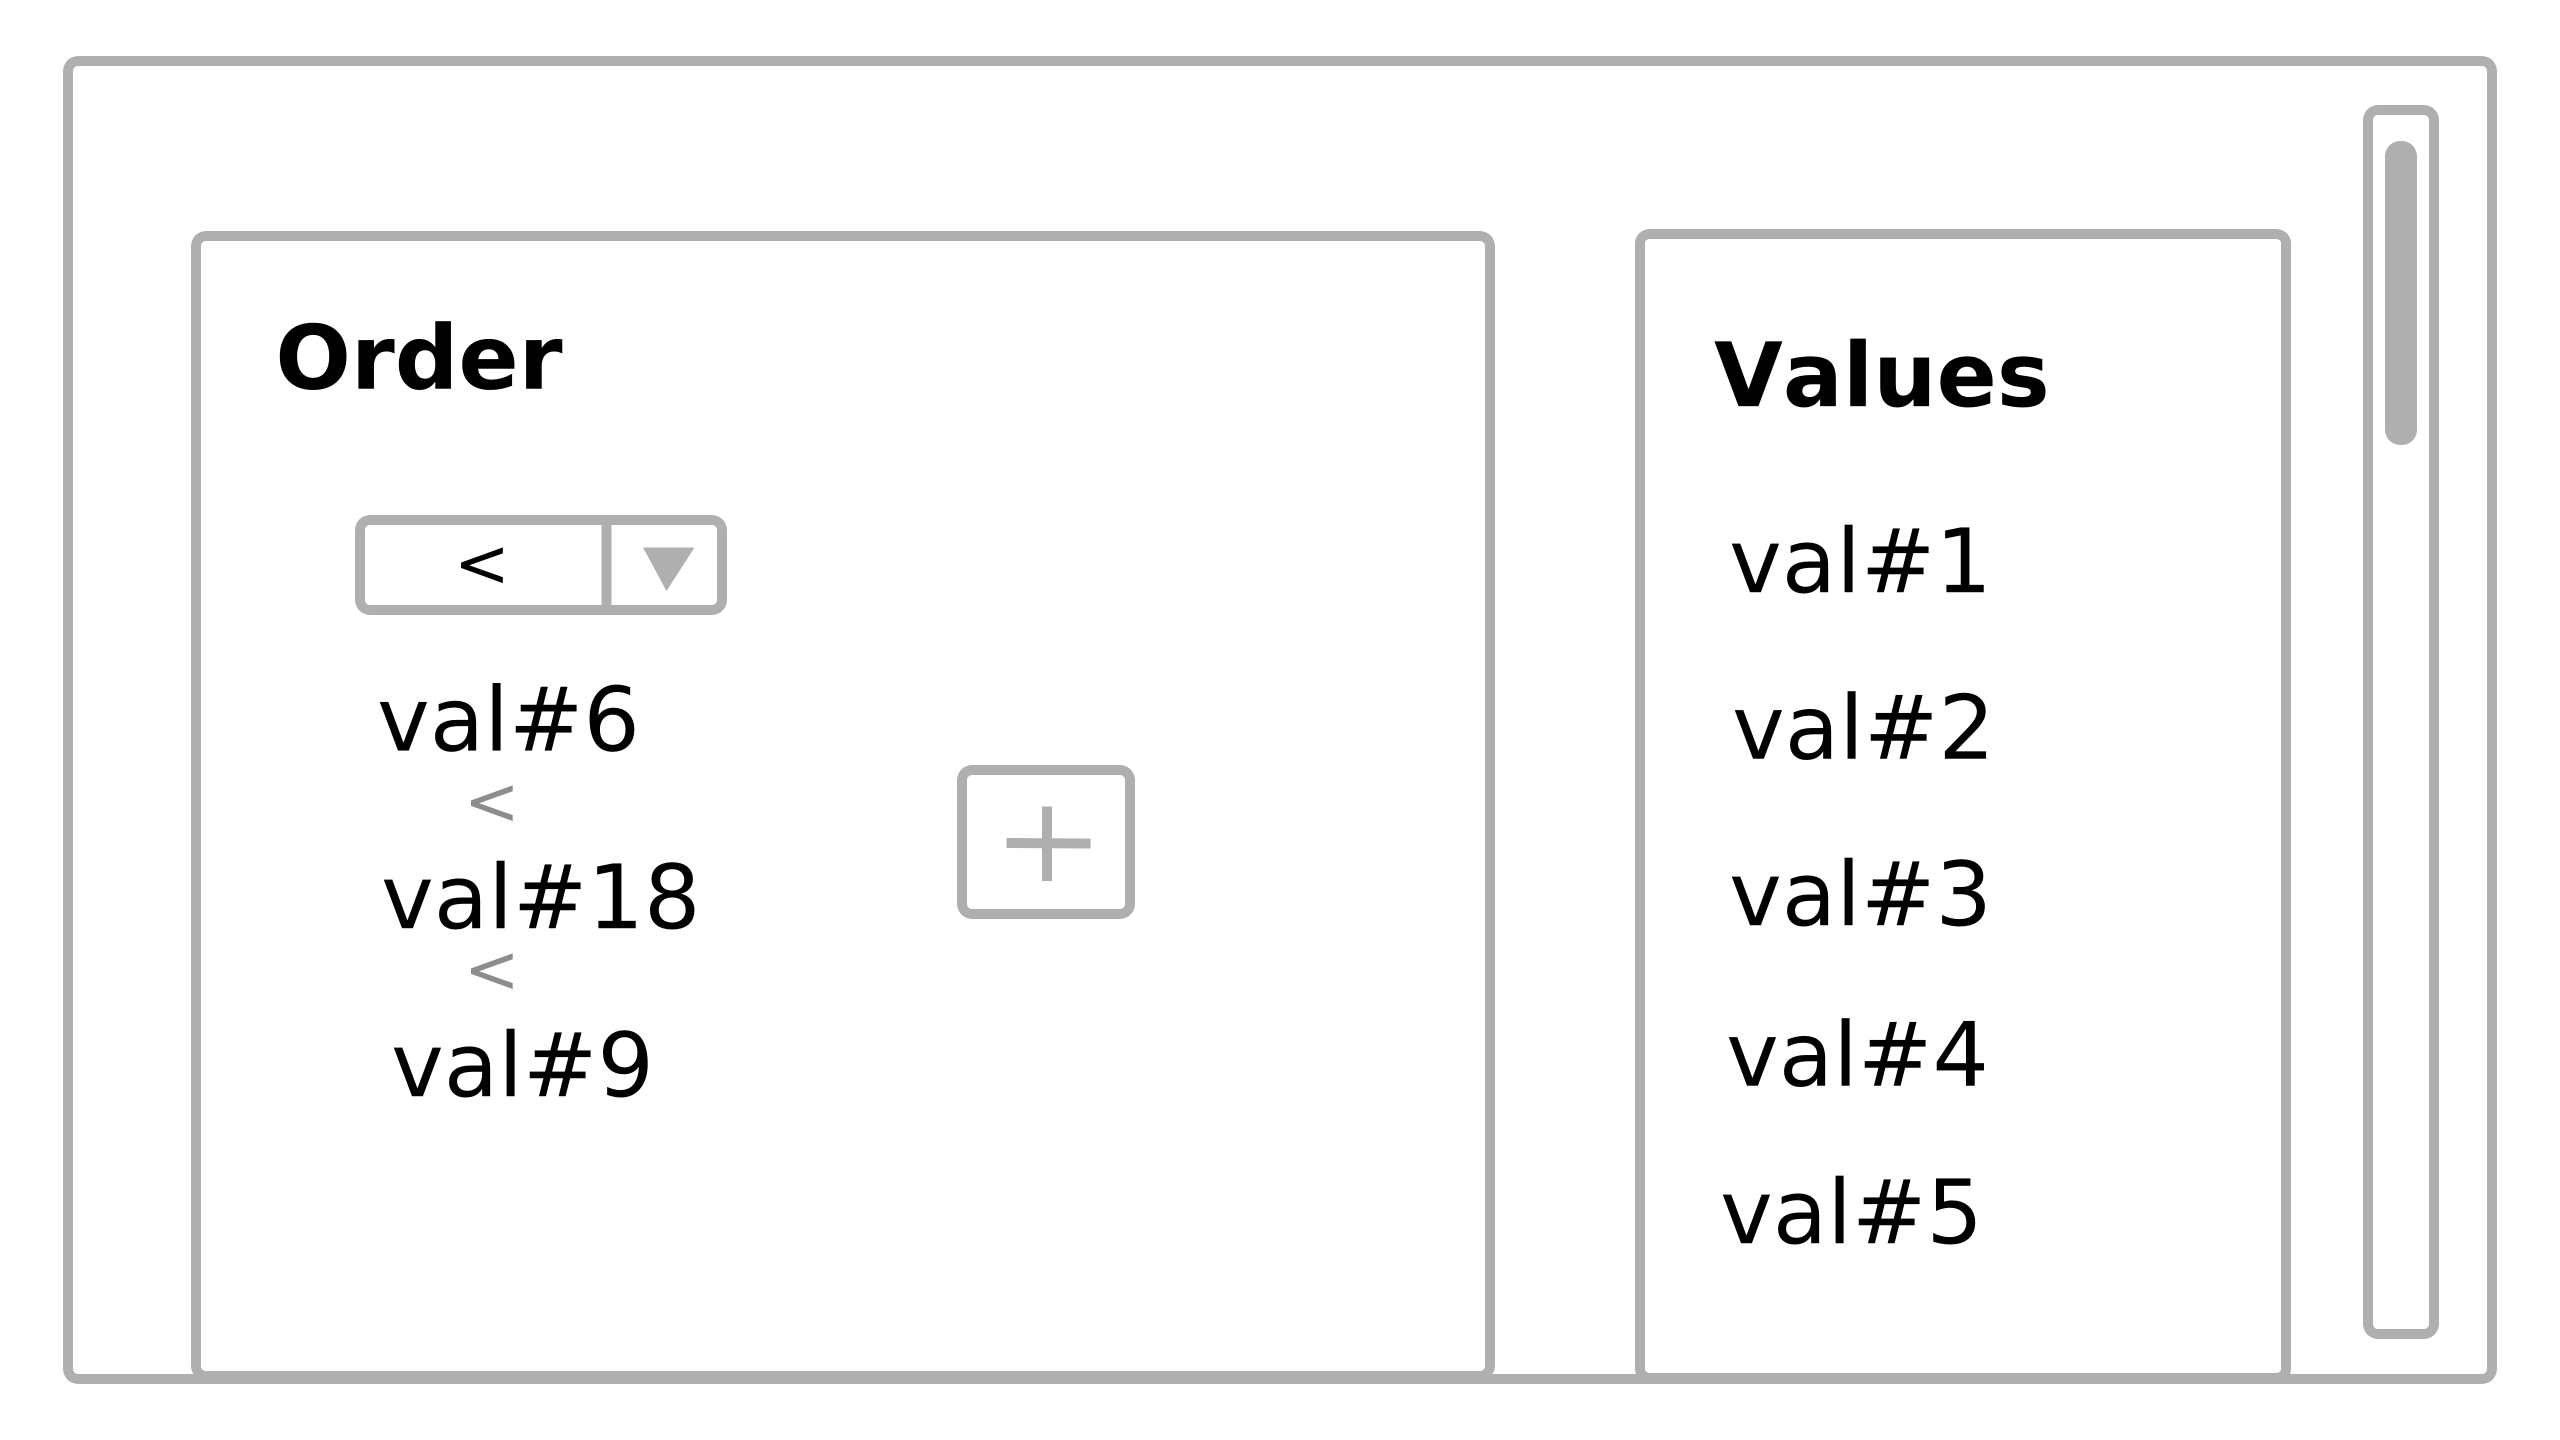
\includegraphics[width=\linewidth]{../mock_up/ord-2.png}
			\caption{Sort with drag and drop}
			\label{fig:p1}
		\end{figure}
	\end{frame}

	\begin{frame}
		\frametitle{Ordinal scaling}
		\begin{figure}[H]
			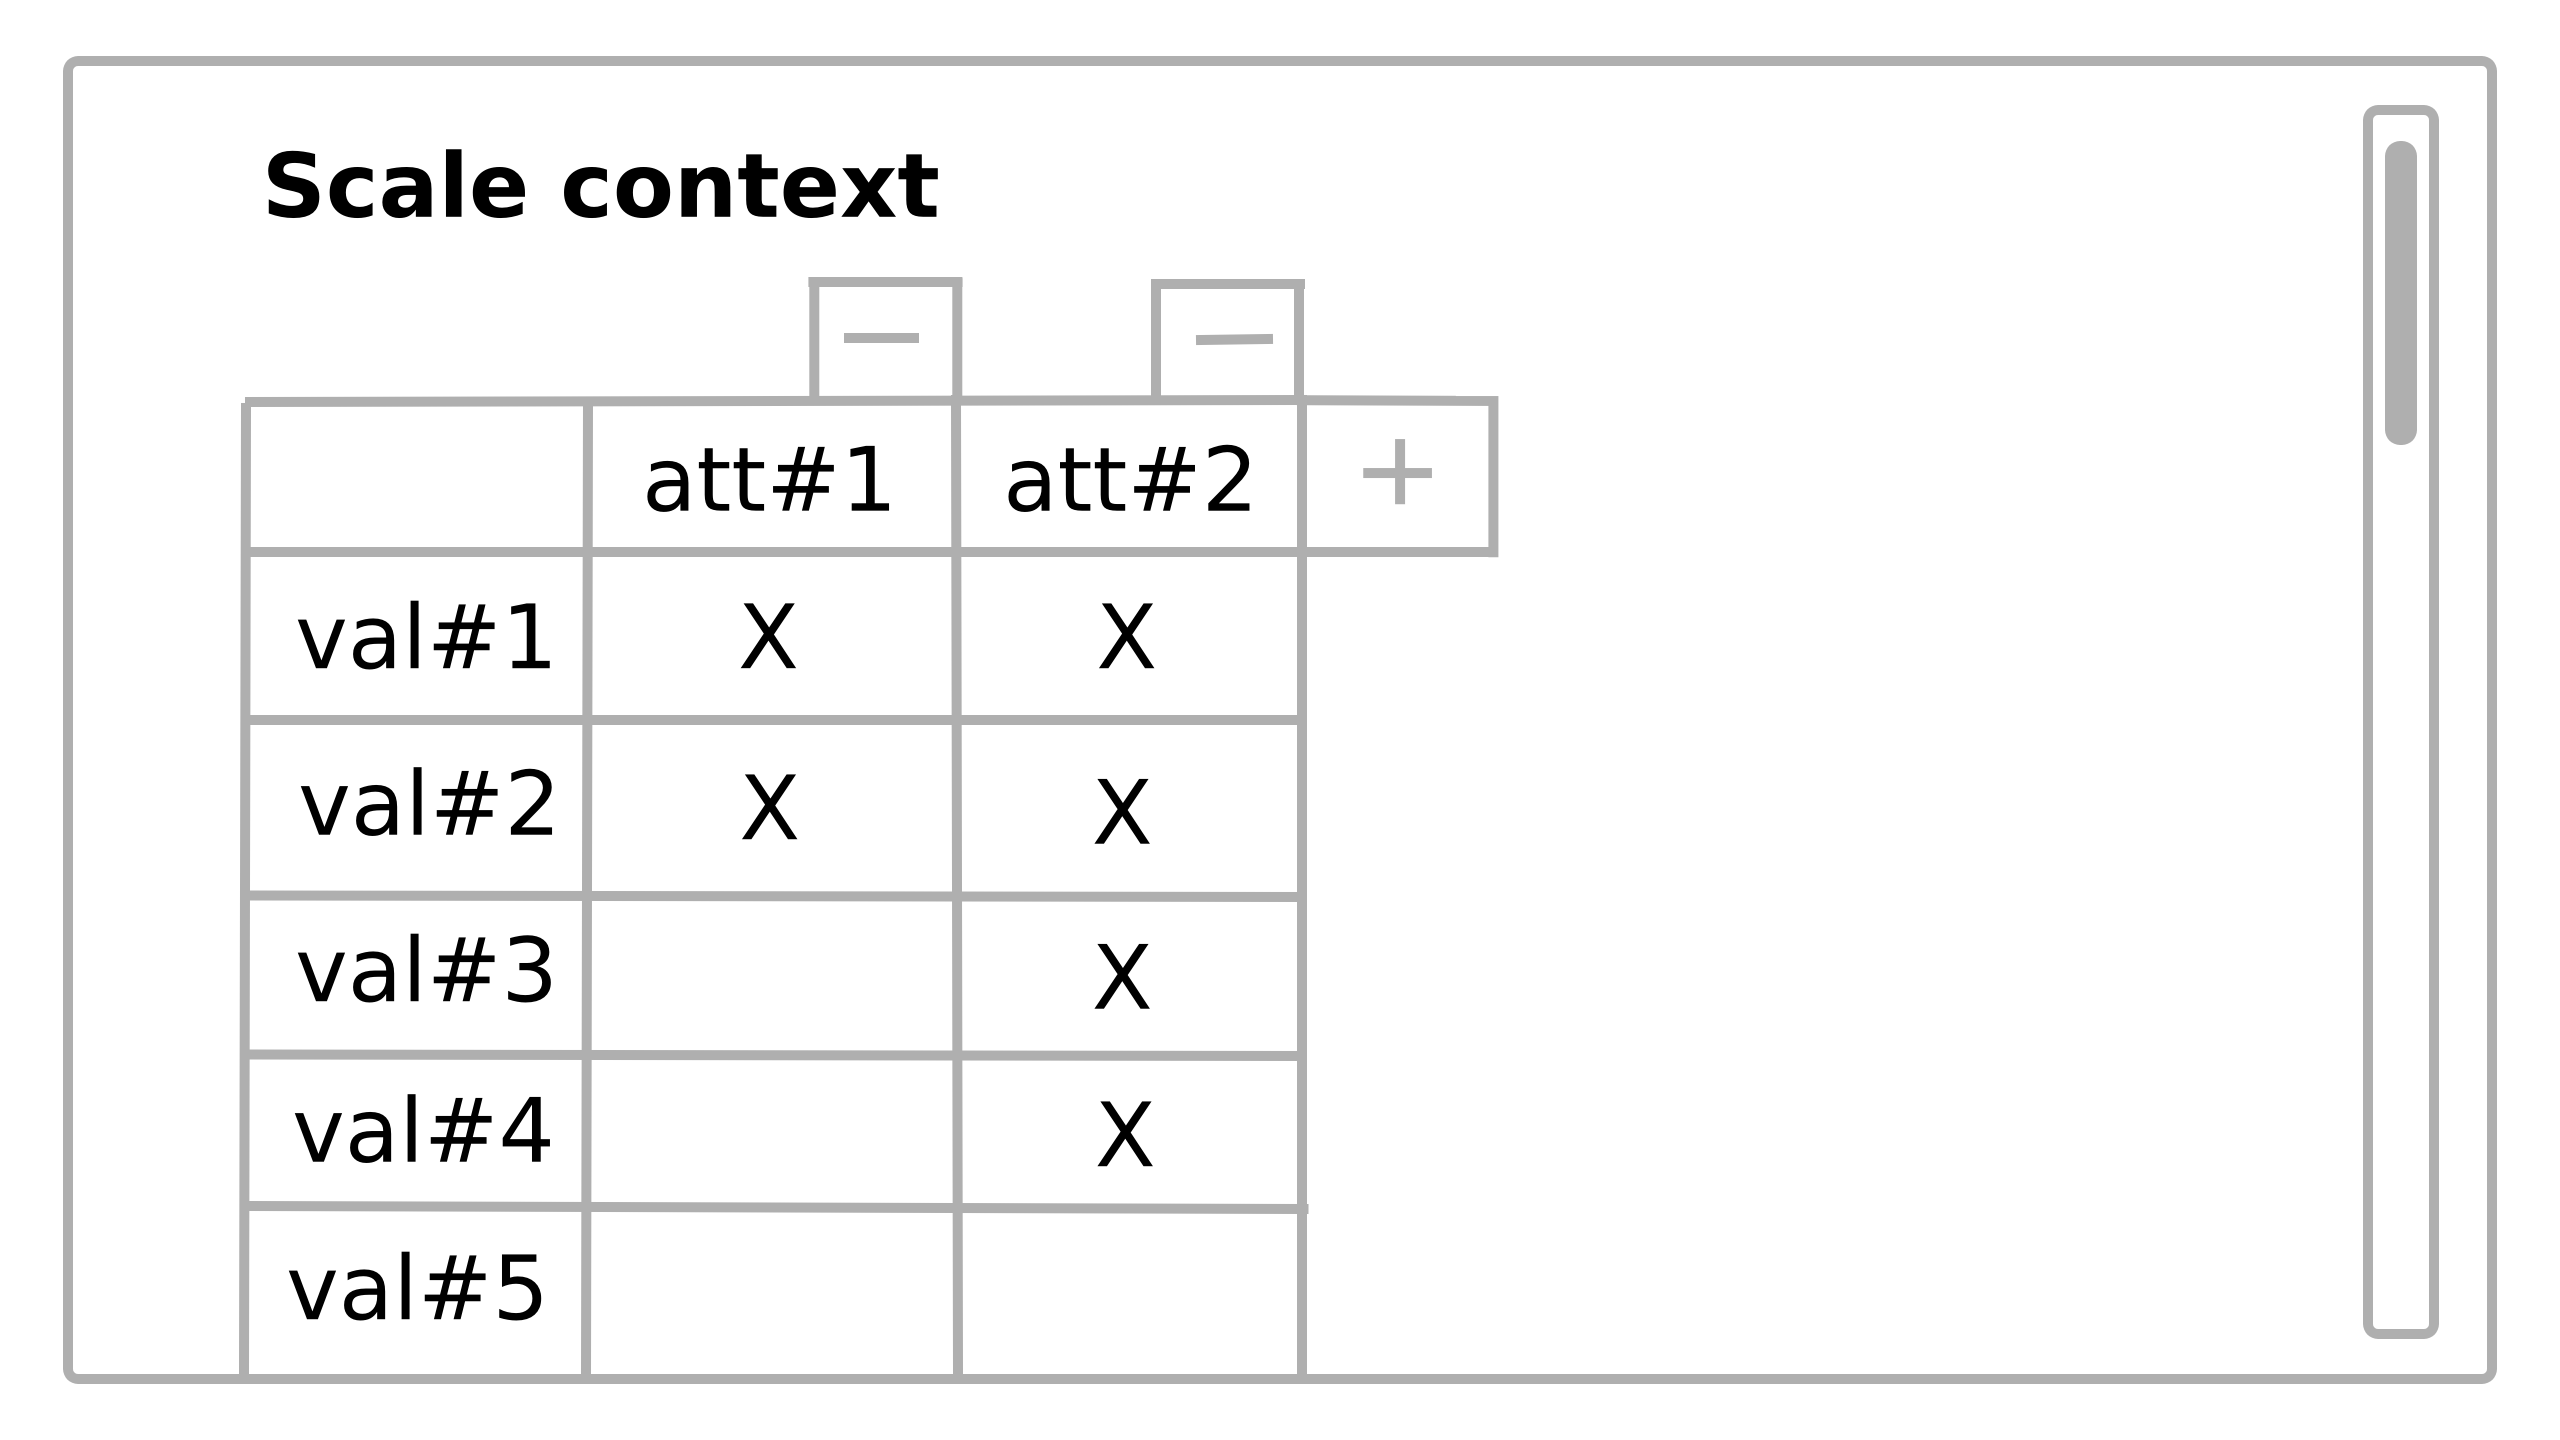
\includegraphics[width=\linewidth]{../mock_up/ord-1.png}
			\caption{Edit the scale directly}
			\label{fig:p1}
		\end{figure}
	\end{frame}

	\begin{frame}
		\frametitle{Numeric scaling}
		\begin{figure}[H]
			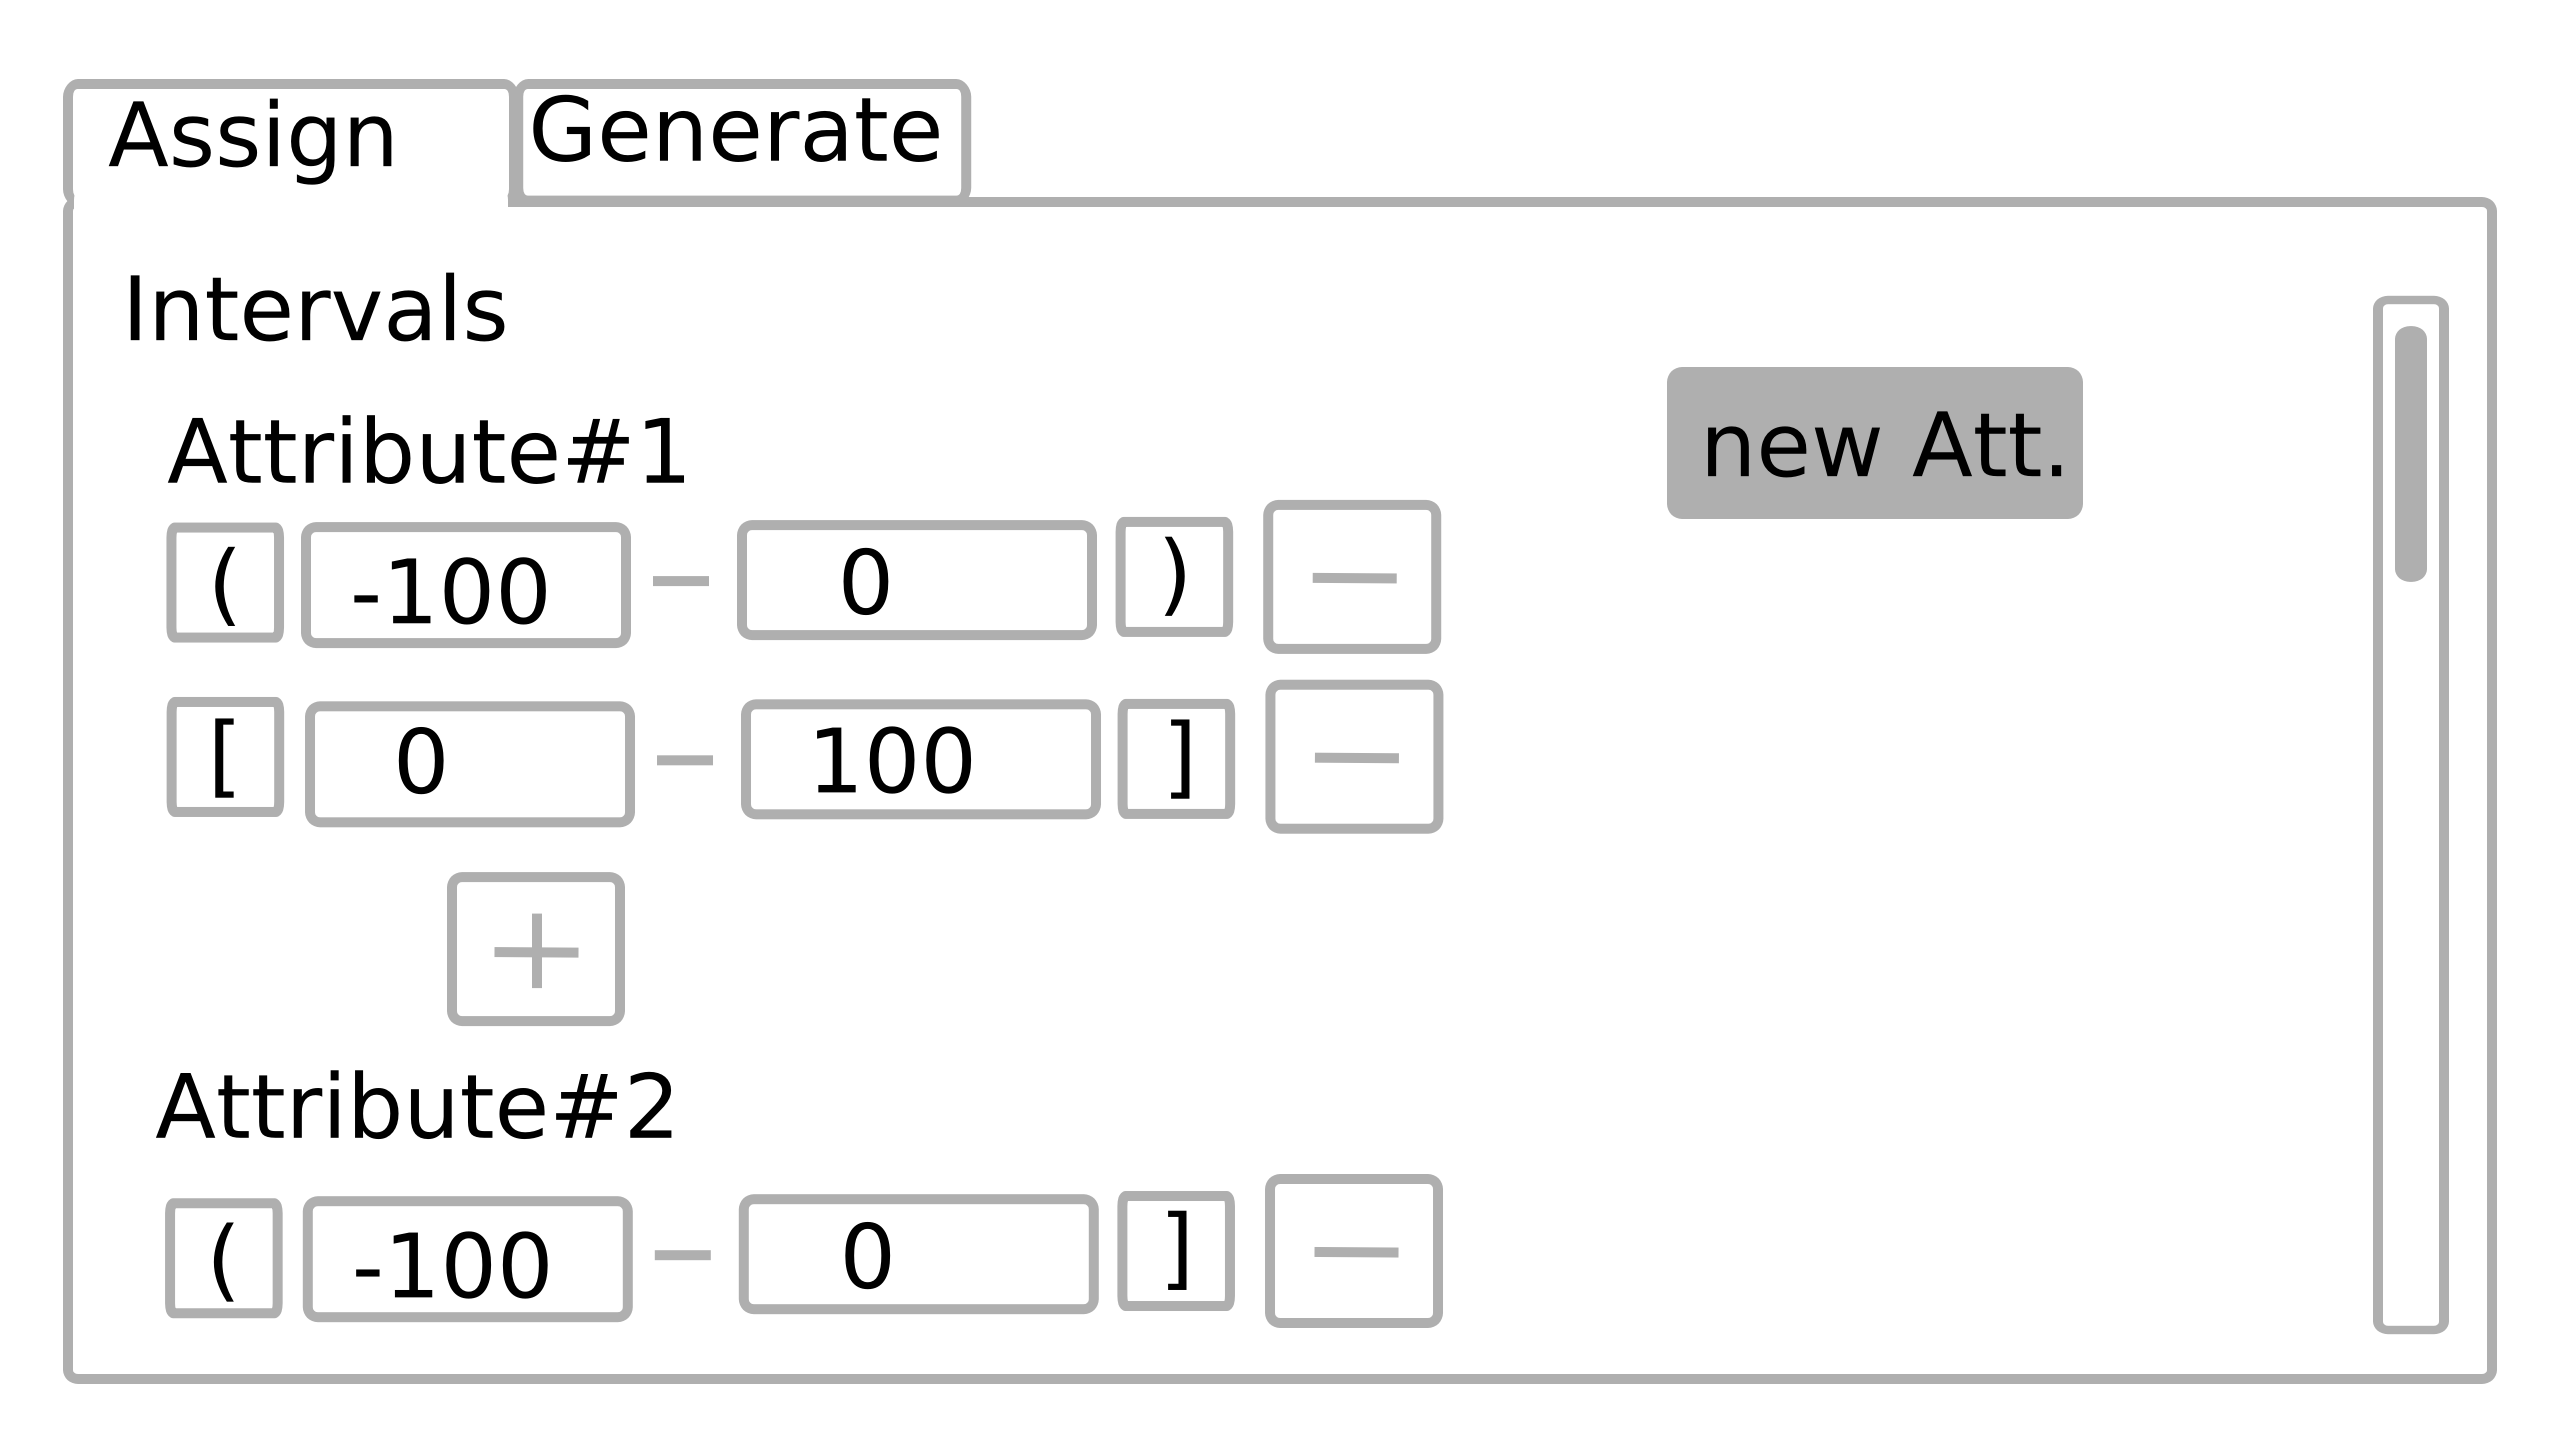
\includegraphics[width=\linewidth]{../mock_up/num.png}
			\caption{Set different intervals per hand}
			\label{fig:p1}
		\end{figure}
	\end{frame}

	\begin{frame}
		\frametitle{Numeric scaling}
		\begin{figure}[H]
			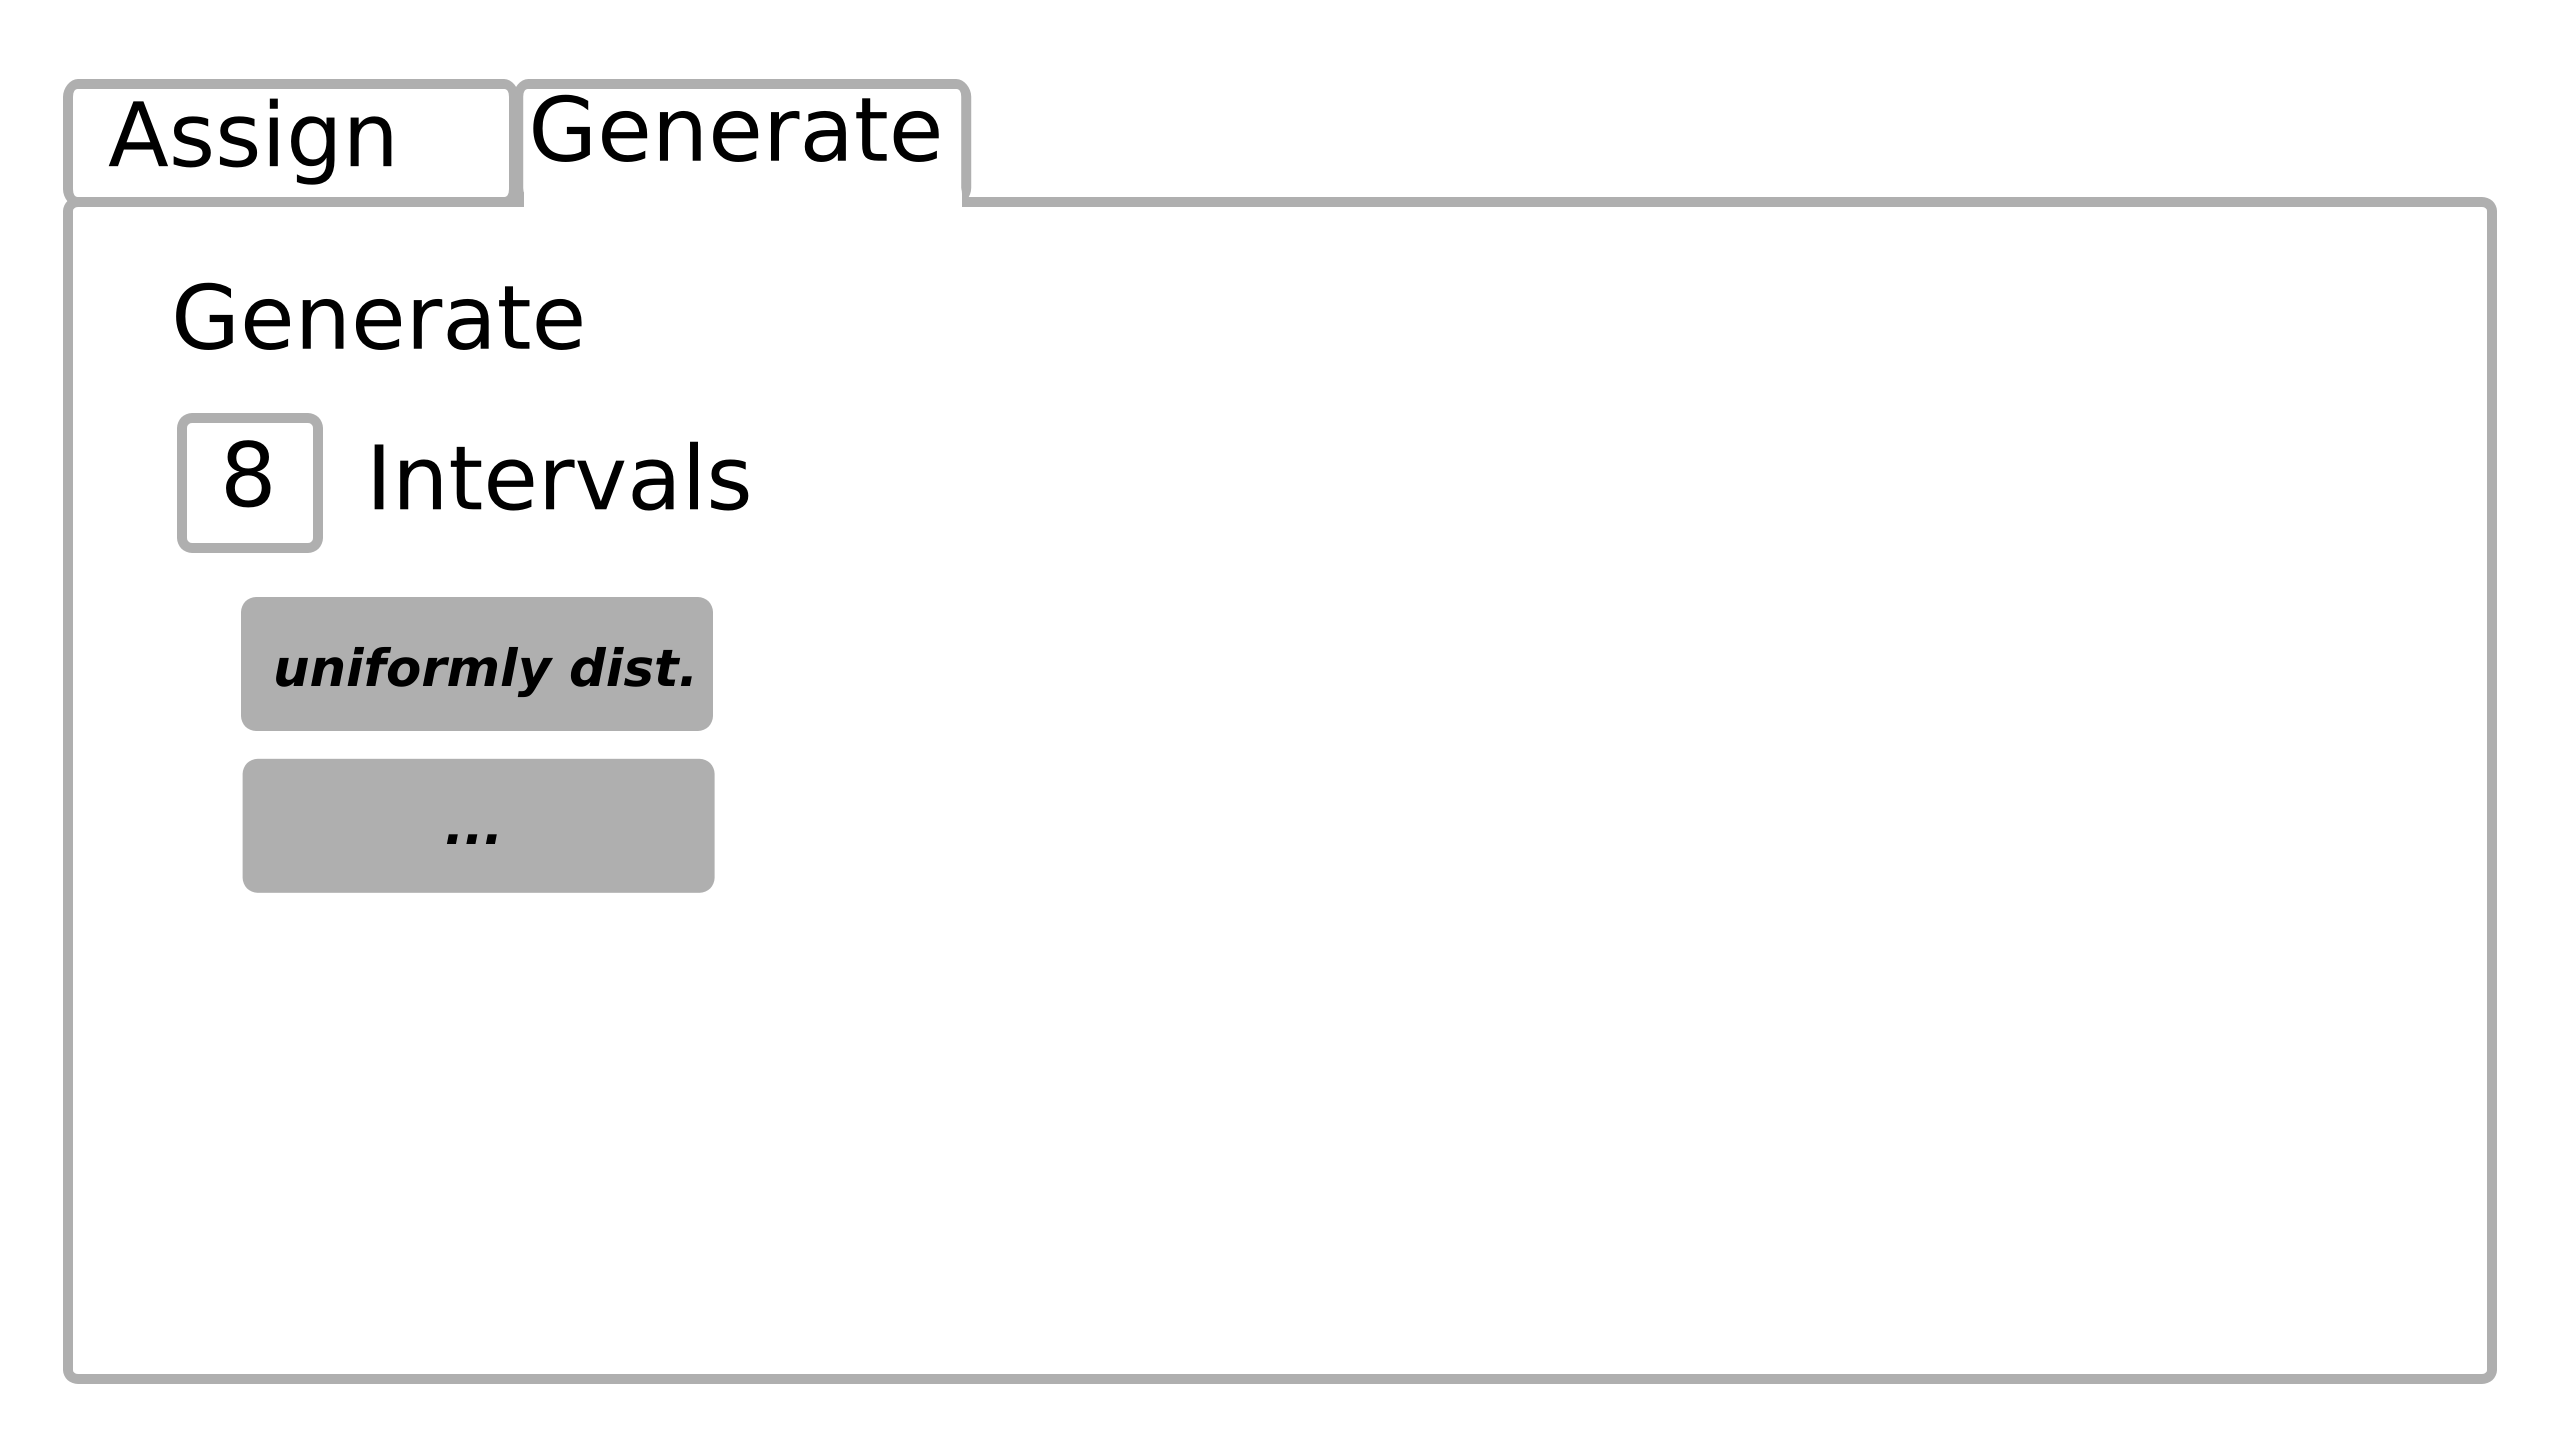
\includegraphics[width=\linewidth]{../mock_up/num_gen.png}
			\caption{Use predefined intervals}
			\label{fig:p1}
		\end{figure}
	\end{frame}

	\begin{frame}
		\frametitle{Export}
		\begin{figure}[H]
			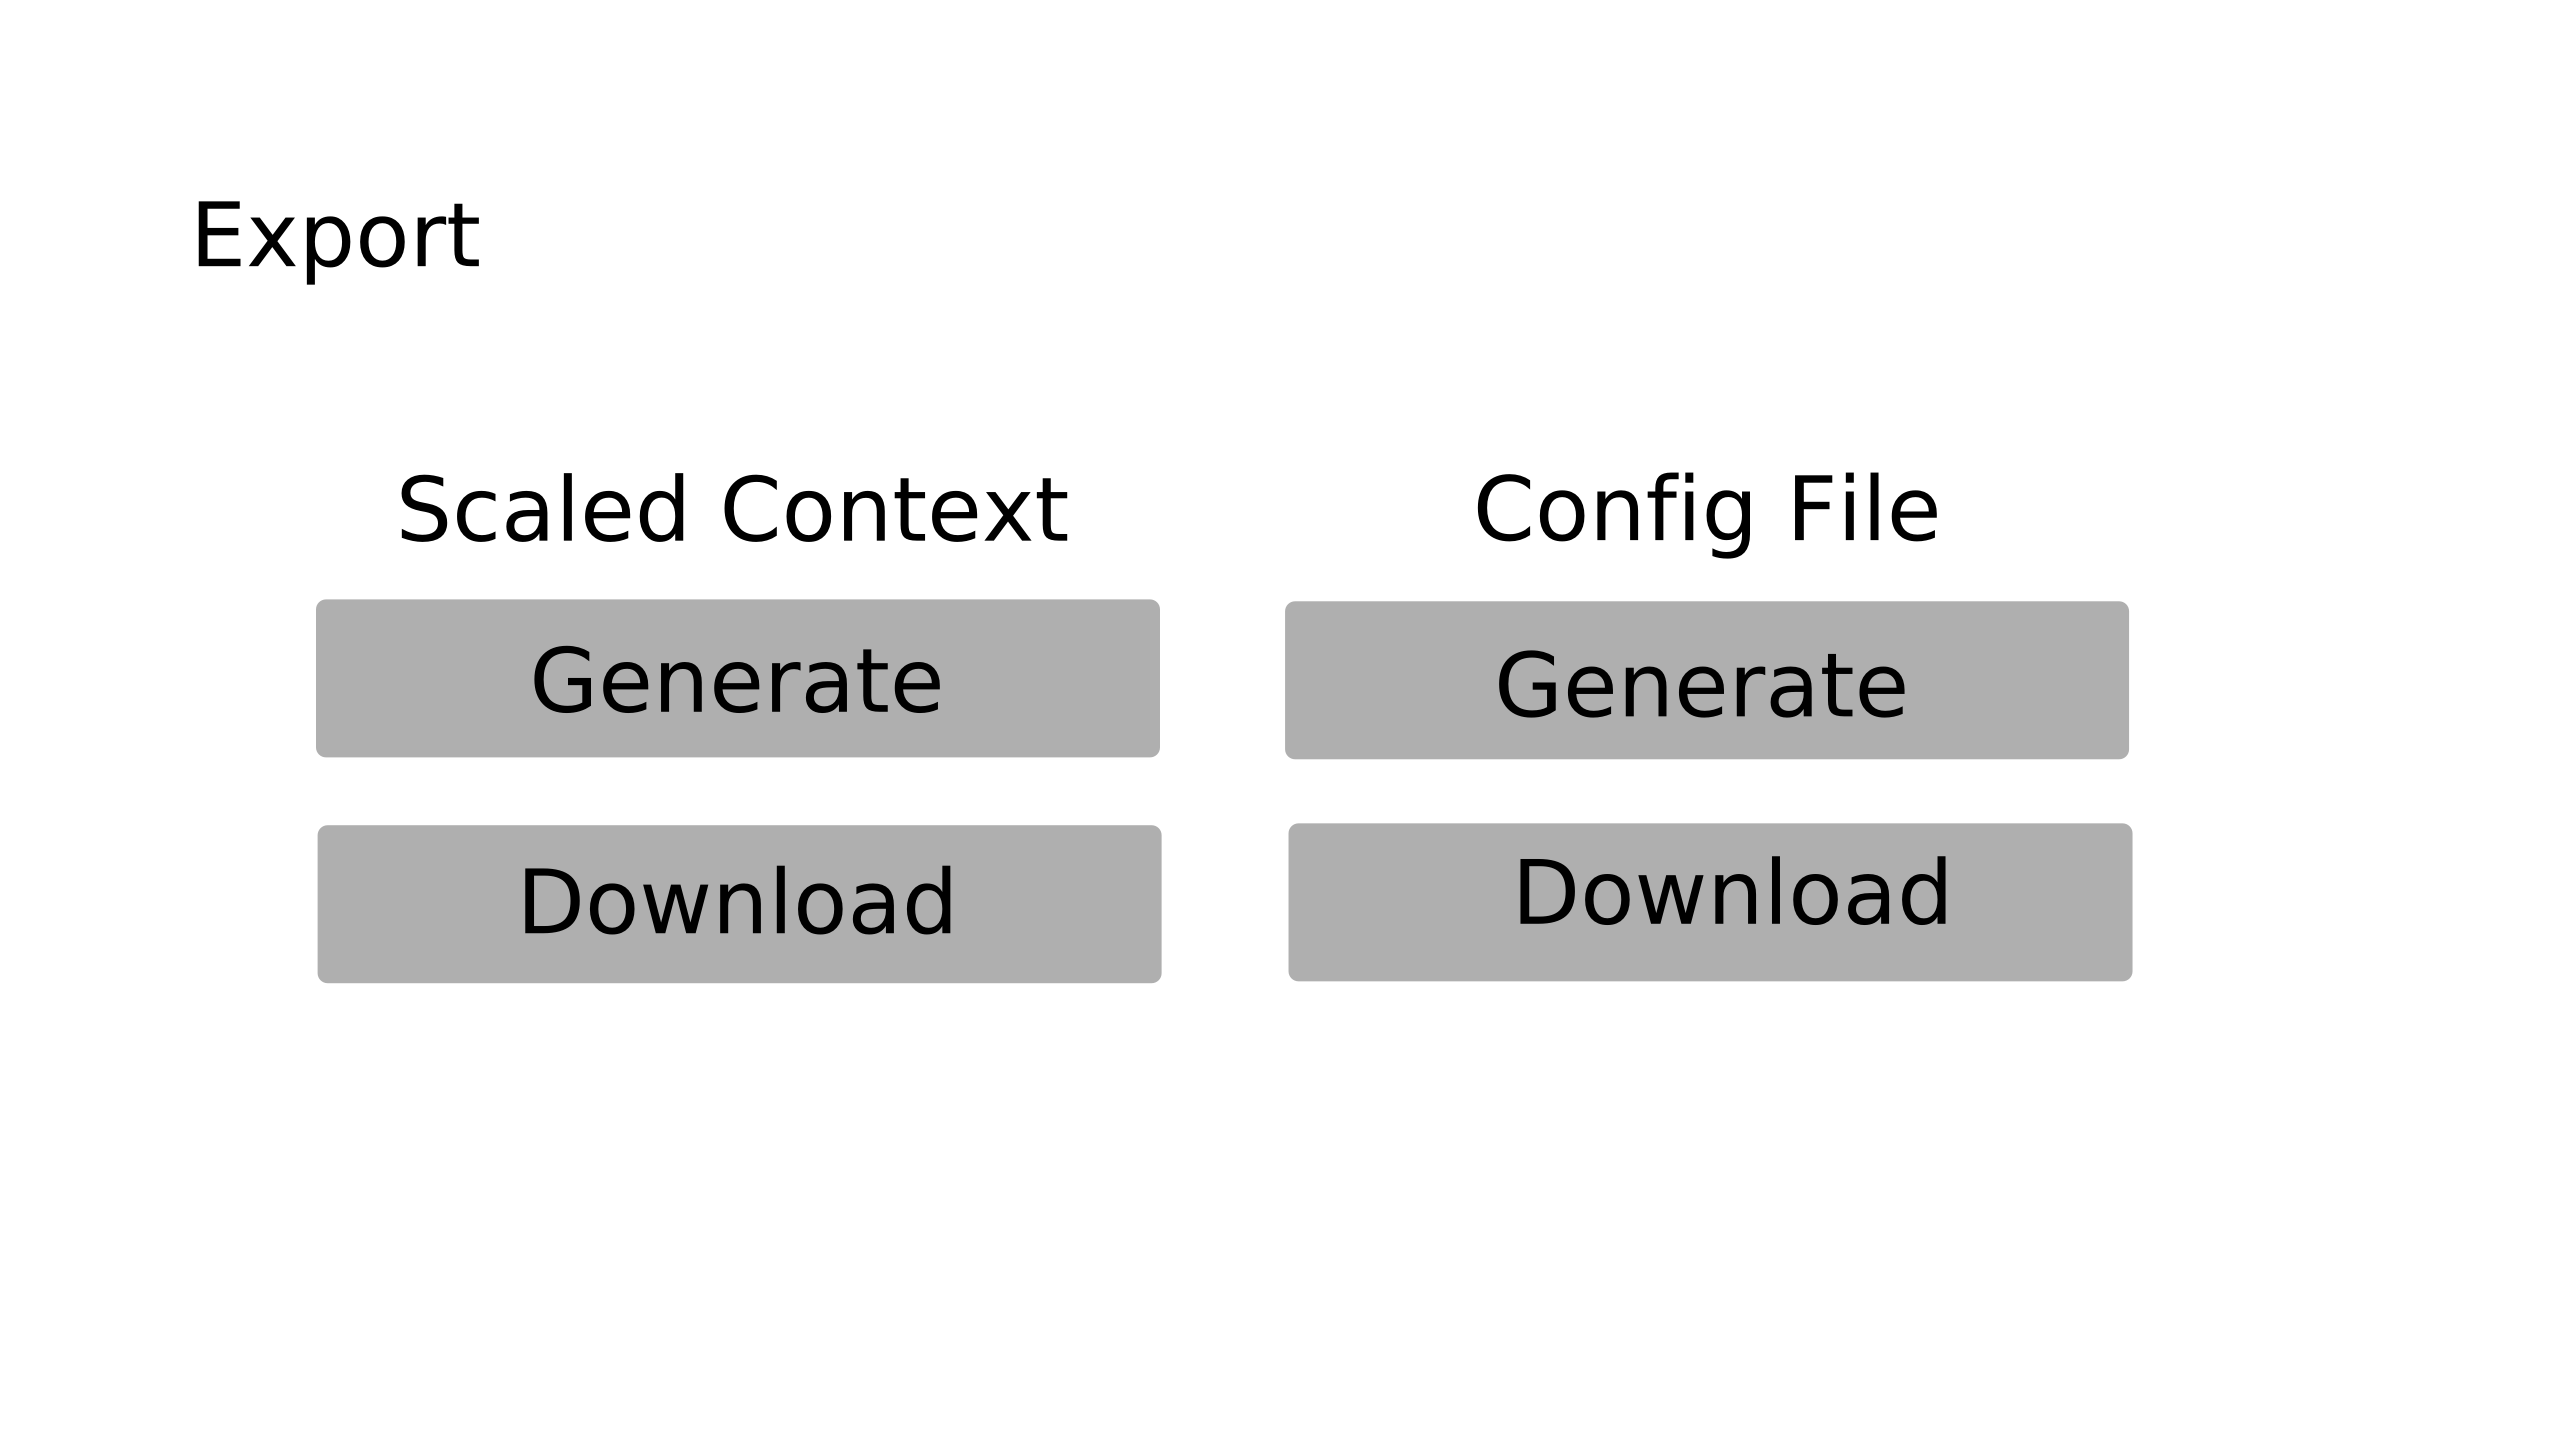
\includegraphics[width=\linewidth]{../mock_up/export.png}
			\caption{Export panel}
			\label{fig:p1}
		\end{figure}
	\end{frame}

\section[]{Live-Demo}

\end{document}
